\documentclass[11pt]{article}

% ---------- Packages ----------
\usepackage[margin=1in]{geometry}
\usepackage{amsmath, amssymb}
\usepackage{graphicx}
\usepackage{fancyhdr}
\usepackage{float}

% ---------- Paragraph Formatting ----------
\setlength{\parindent}{0pt}
\setlength{\parskip}{0.5em}

% ---------- Header ----------
\pagestyle{fancy}
\fancyhf{}
\lhead{ASEN 5090 Introduction to GNSS}
\rhead{Justin Le}
\cfoot{\thepage}

% ---------- Document ----------
\begin{document}

% ---------- Title ----------
\begin{center}
    {\Large \textbf{Homework 1}}\\[0.5em]
    {\large ASEN 5090 Introduction to GNSS}\\[0.5em]
    Justin Le\\
    \today
\end{center}

\vspace{1em}

% ============================================================
% Problem 1
% ============================================================

\section*{Problem 1}

\subsection*{(a)} 
 PL1 = 550 [m] \newline
 PL2 = 500 [m]

\begin{figure}[htbp]
    \centering
    % \includegraphics[width=0.7\textwidth]{figure_name.png}
    \caption{Insert figure caption here.}
    \label{fig:problem1}
\end{figure}

Let
\[
\rho^{k}=\sqrt{(x^{k}-x)^2+(y^{k}-y)^2+(z^{k}-z)^2}+b.
\]

Given the setup, this can be constrained to a 1D problem on the $x$ axis,
\[
\rho^{k}=\sqrt{(x^{k}-x)^2}+b.
\]

Which is equivalent to,
\[
\rho^{k}=|(x^{k}-x)|+b.
\]

Given the setup on a line, we have the $\rho^{1}$, the observed position be $550m$, and $x^{1}$ 
position on the line being 0. Likewise $\rho^{2}=500m$ and $x^{2}=1000m$.
This gives a set of equations

PL1:
\[
\begin{aligned}
550m &= |0-x|+b \\
550m &= x+b
\end{aligned}
\]

PL2:
\[
\begin{aligned}
500m &= |1000m-x|+b \\
-500m &= -x+b
\end{aligned}
\]

This can be solved by elimination, eliminating the bias $b$ giving,
\[
1050m = 2x
\]
\[
\boxed{\therefore\quad x = 525\,[m]}
\]

Rewrite the PL1 equation to solve for $b$.
\[
\boxed{
\begin{aligned}
b &= 550m-x \\
\therefore\quad b &= 25\,[m]
\end{aligned}
}
\]


\subsection*{b.}

\[
\begin{aligned}
\text{PL1} &= 400\,[m] \\
\text{PL2} &= 1400\,[m]
\end{aligned}
\]

The solution method remains the same, where we develop a system of equations from 
the observed ranging measurements and based on the known locations of the sat.

PL1:
\[
\begin{aligned}
400m &= |x|+b \\
\end{aligned}
\]

PL2:

\[
\begin{aligned}
1400m &= |1000-x|+b
\end{aligned}
\]

And with eliminaton and eliminating $x$ this time, we obtain,
\[
\begin{aligned}
800m = 2b \\
\boxed{\therefore b = 400 [m]}
\end{aligned}
\]

And solve for $x$ with 
\[
\begin{aligned}
x = b-400 \\
\boxed{\therefore x = 0}
\end{aligned}
\]

\section*{Problem 2}

\subsection*{(a)}

\begin{figure}{htbp}
\centering
% \includegraphics[width=0.7\textwidth]{figure_name.png}
\caption{Insert figure caption here.}
\label{fig:problem2}
\end{figure}

From the diagram above, we are able to create solve for the
following equations as functions of $x_{a}, v_{0}, h_{0}$.
\[
\begin{aligned}
R(x_{a}, v_{0}, h_{0}) \\
\dot{R}(x_{a}, v_{0}, h_{0}) \\
z(x_{a}, v_{0}, h_{0})
\end{aligned}
\]

When solving for range, one can simply use the pythagorean
theorum given $h_{0}$ is constant.
\[
\boxed{ R = \sqrt{x_a^2 + h_0^2} }
\]

Solving for range rate, take the differential w.r.t time.

\[
\begin{aligned}
R &= \sqrt{x_a^2+h_0^2} \\[2pt]
\dot{R}
  &= \frac{dR}{dt} \\
  &= \frac{1}{2}\left(x_a^2+h_0^2\right)^{-1/2}
     \left(2x_a\dot{x}_a+2h_0\dot{h}_0\right) \\
  &= \frac{x_a\dot{x}_a+h_0\dot{h}_0}
     {\sqrt{x_a^2+h_0^2}}
\end{aligned}
\]

Since $h_0$ is constant, $\dot{h}_0=0$, and $\dot{x}_a=v_0$:

\[
\boxed{
\dot{R}
= \frac{x_a v_0}{\sqrt{x_a^2+h_0^2}}
}
\]

Solving for zenith, looking at the diagram, finding $z$ as a function of $x_a$
can simply be

\[
\boxed{z = \arctan( \frac{x_a}{h_0})}
\]


\subsection*{(b.)}

See attached MATLAB script. 

\begin{figure}[H]
    \centering
    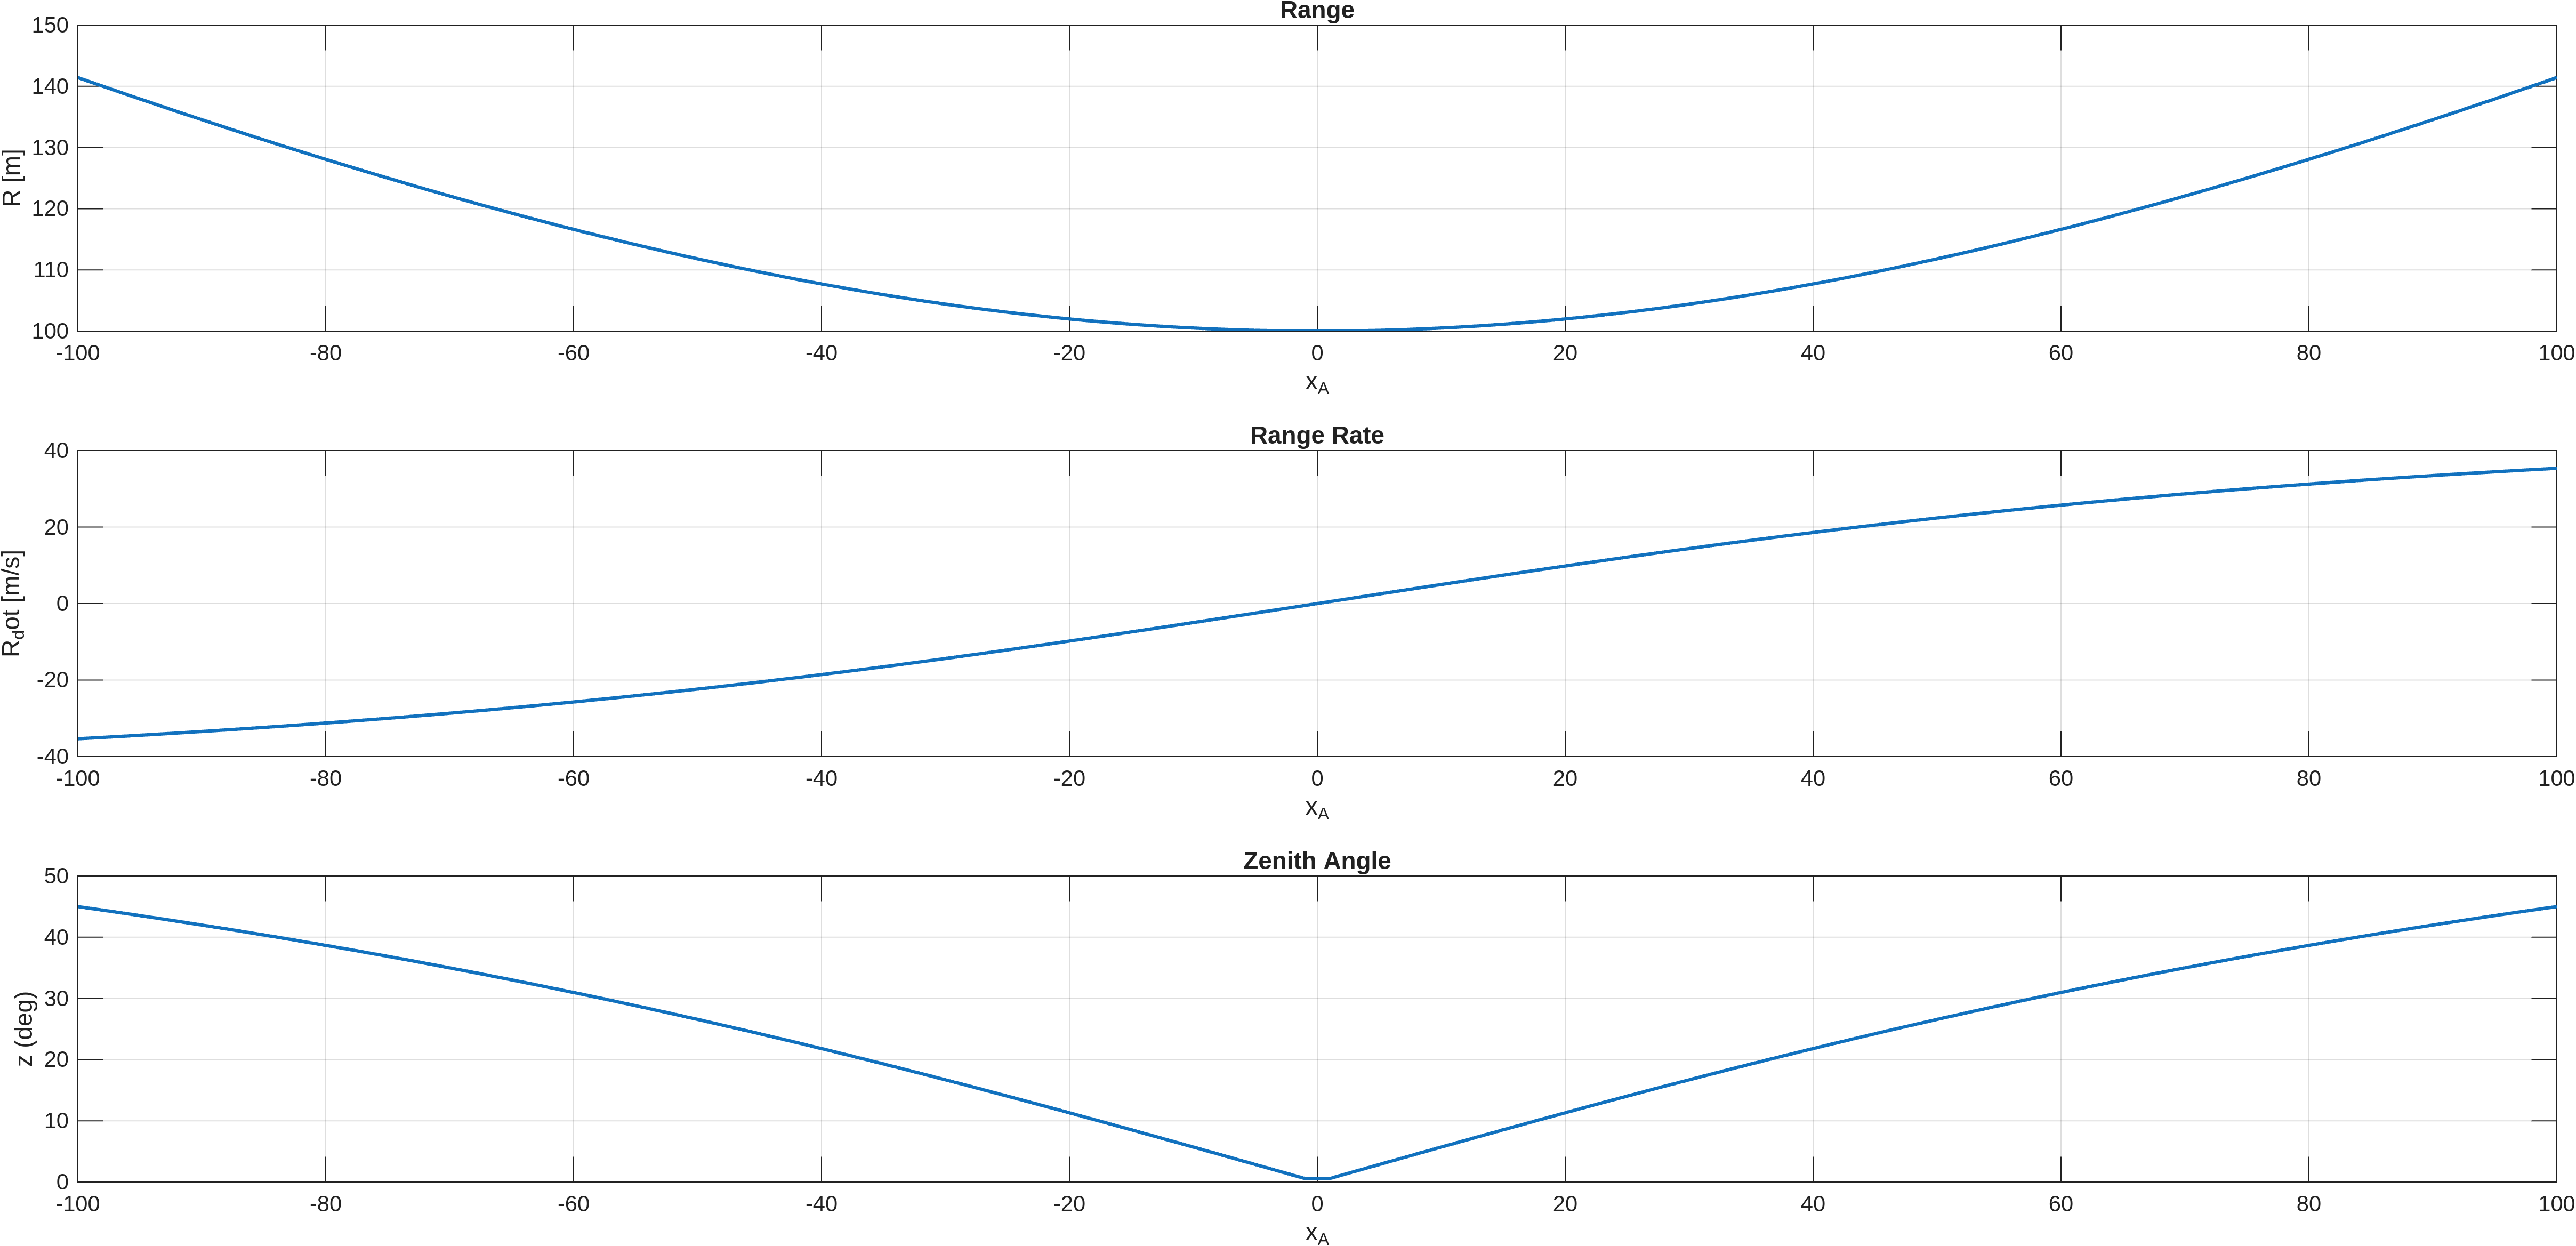
\includegraphics[width=0.8\textwidth]{../HW1_sensitivity.png}
    \caption{MATLAB Script Results}
    \label{fig:sensitivity}
\end{figure}


\subsection*{(c.)}
\hspace*{2em}The three types of measurements for determining $x_a$ varies. 
Taking a look at the sensitivity of each measurement compared to the
aircraft position. We see that there is different slopes at these 
different aircraft postitions, when farther away from the ground station,
Range rate and Zenith angle's slopes are more gradual, leading to less sensitivity.
However when closer to the ground station, the pattern changes where Range rate
and Zenith angle would have more steep slopes and be more sensitive. This is 
opposed to Range, where when close the ground station it would be less sensitive
and more useful in this section.

\subsection*{(d.)}
\begin{figure}[H]
    \centering
    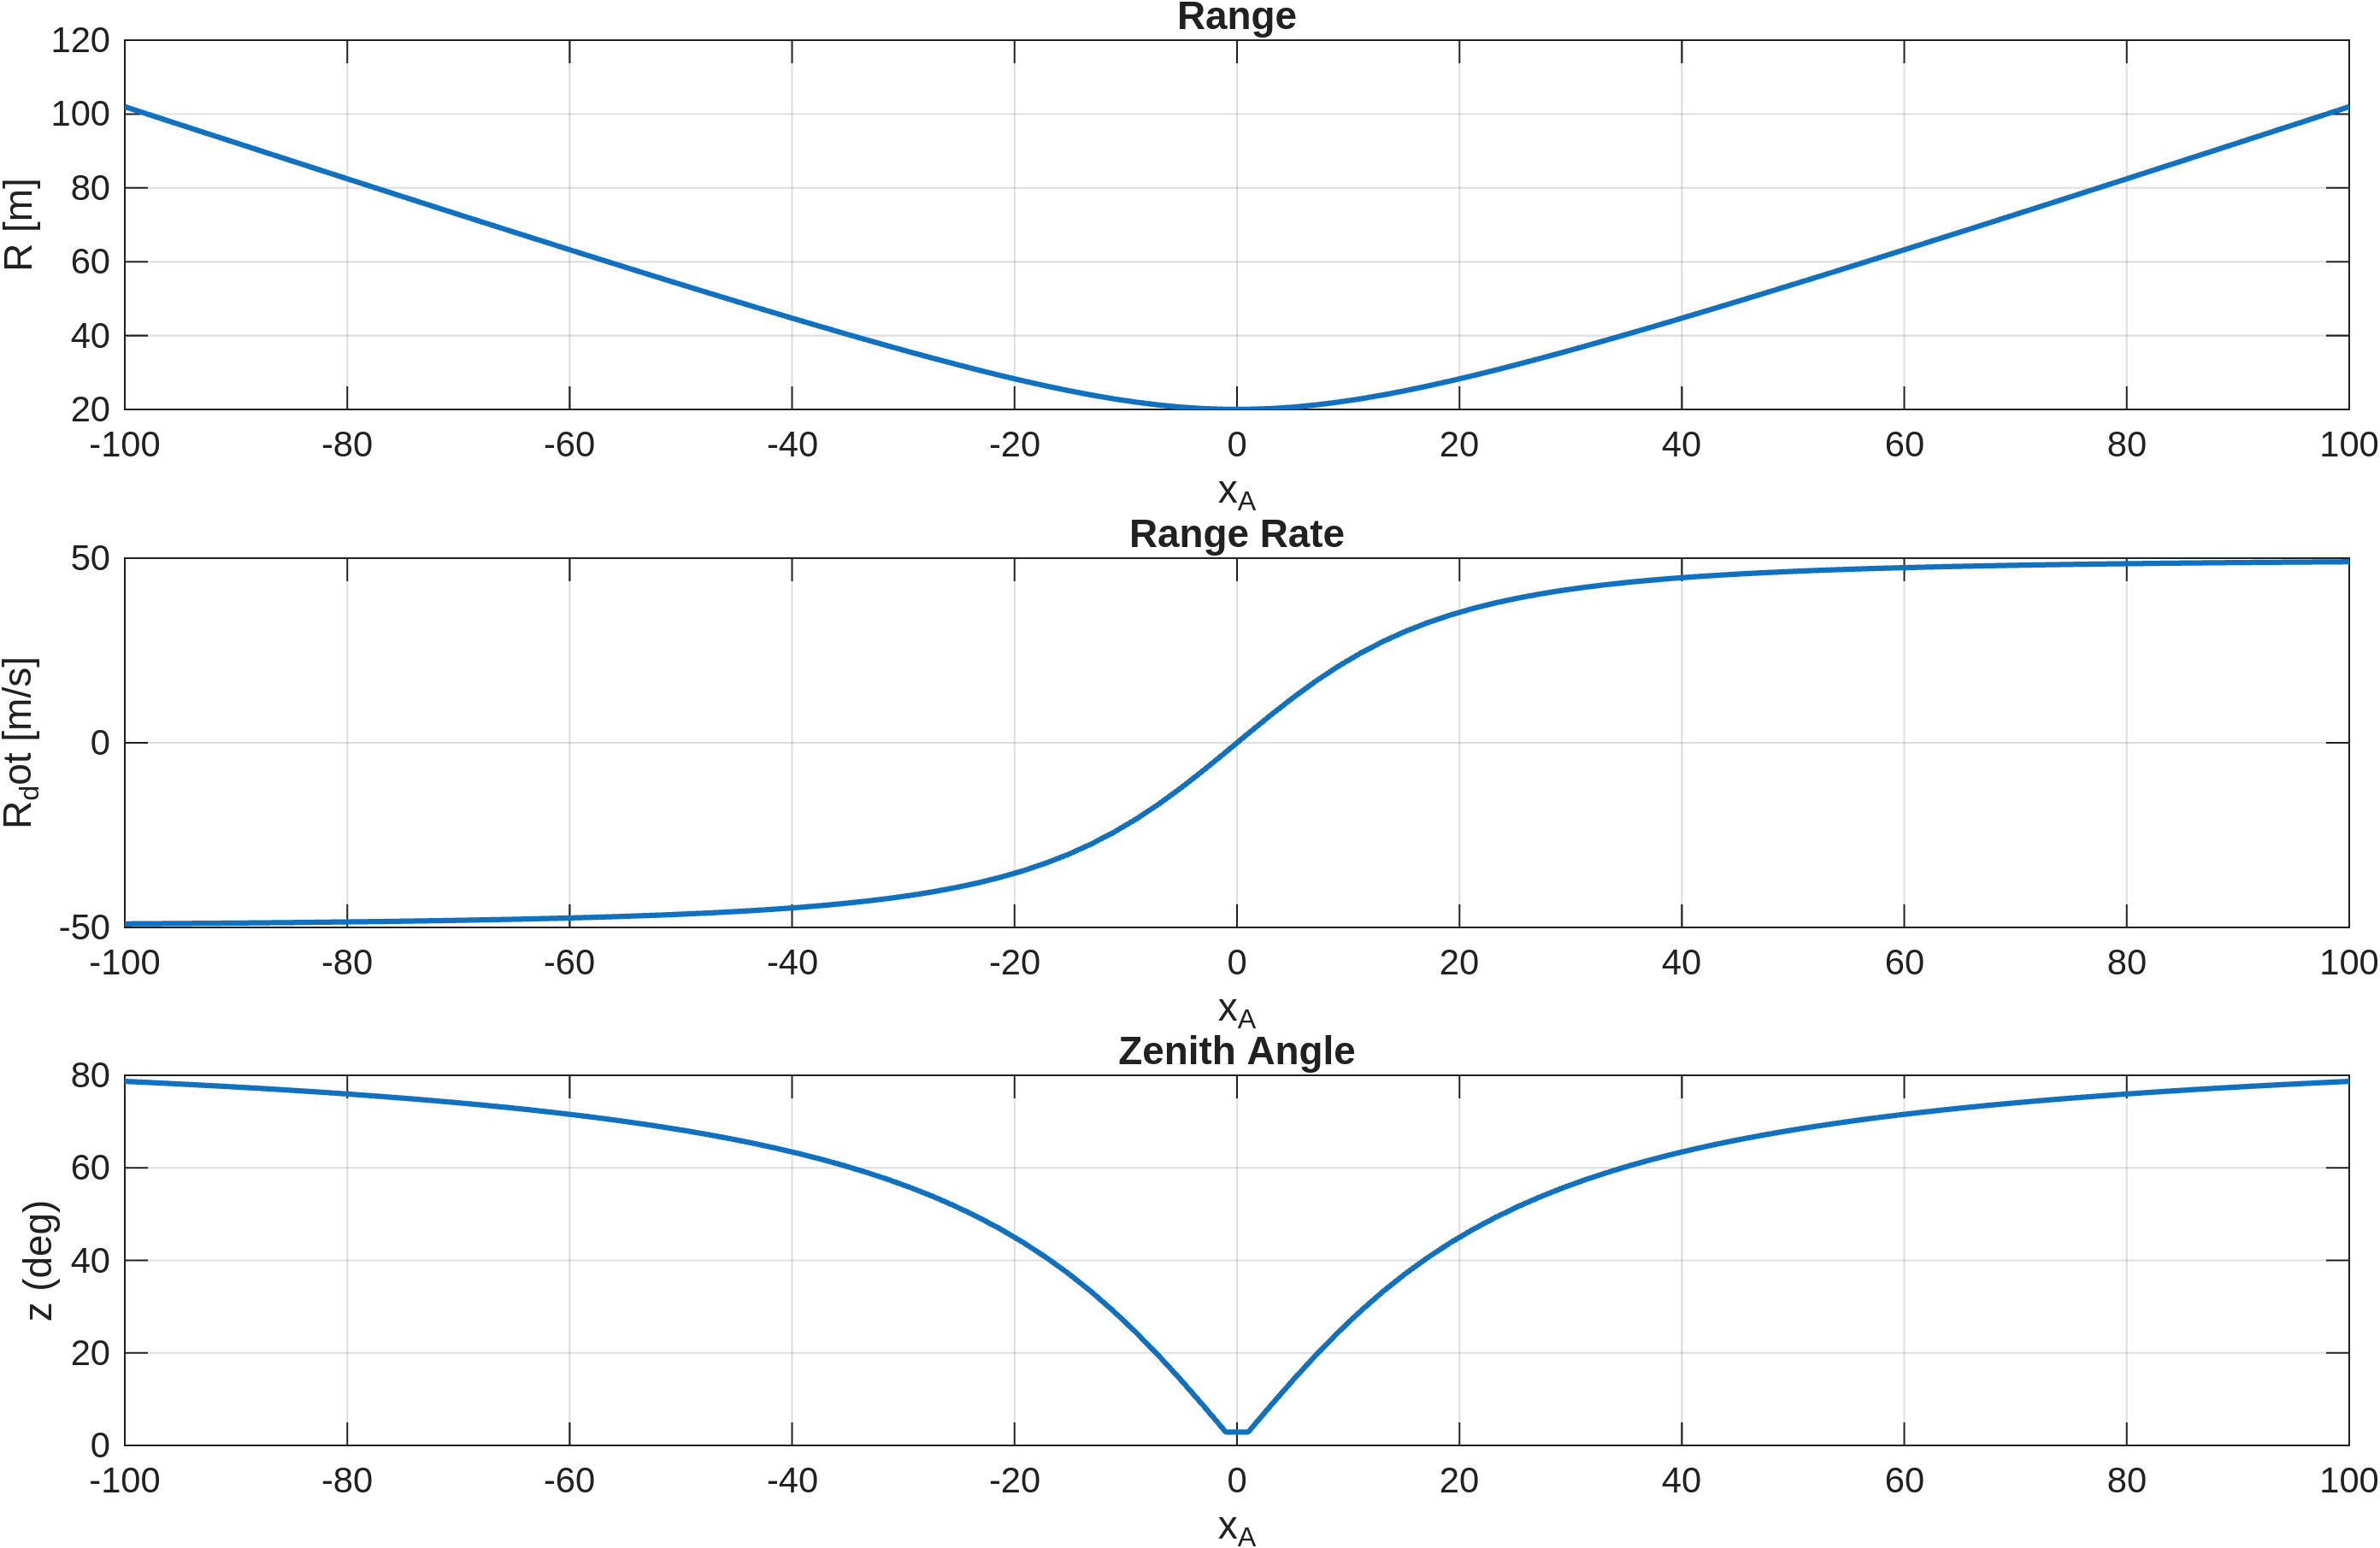
\includegraphics[width=0.8\textwidth]{../HW1_sensitivity_low_alt.png}
    \caption{MATLAB Sensitivity at Lower Altitude}
    \label{fig:sensitivity low alt}
\end{figure}

\hspace*{2em}The sensitivity/utility of the observations at a lower altitude
would depend on the parameter being examined and aircraft position. Taking a look at Figure \ref{fig:sensitivity low alt}, we can 
see the change in behavior, where when further away from the ground
station, there is more sharper slopes for Range, but more smooth behavior
from Range Rate and Zenith Angle. The is inverted as the aircraft gets closer
to the ground station.

\section*{Problem 3}

\subsection*{(a.)}

\begin{figure}[H]
    \centering
    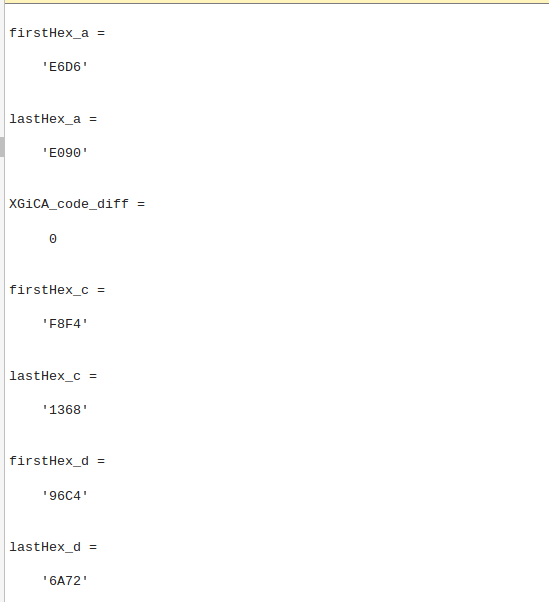
\includegraphics[width=0.8\textwidth]{../hex_console_results.png}
    \caption{MATLAB C/A Code Generation Results}
    \label{fig:CA code gen results}
\end{figure}

When examning the outputs for the first 16 chips expressed
in hex, we do indeed obtain E6D6.

\subsection*{(b.)}
When we create the C/A code form 1024 to 2046, we actually obtain
the same code as we did in part (a.). This can be verified by taking 
the difference between the two vectors and then finding summing up
all the elements, we obtain 0. This means they are identical. 

\subsection*{(c.)}
Repeating what we do for (a.), we are able to verify that it is the 
correct C/A code generated with the first 16 chips expressed in hex 
to be F8F4.

\subsection*{(d.)}
Repeating what we do for (a.), we are able to verify that it is the 
correct C/A code generated with the first 16 chips expressed in hex 
to be 96C4.

\section*{Problem 4}
\subsection*{(a.)}

\begin{figure}[H]
    \centering
    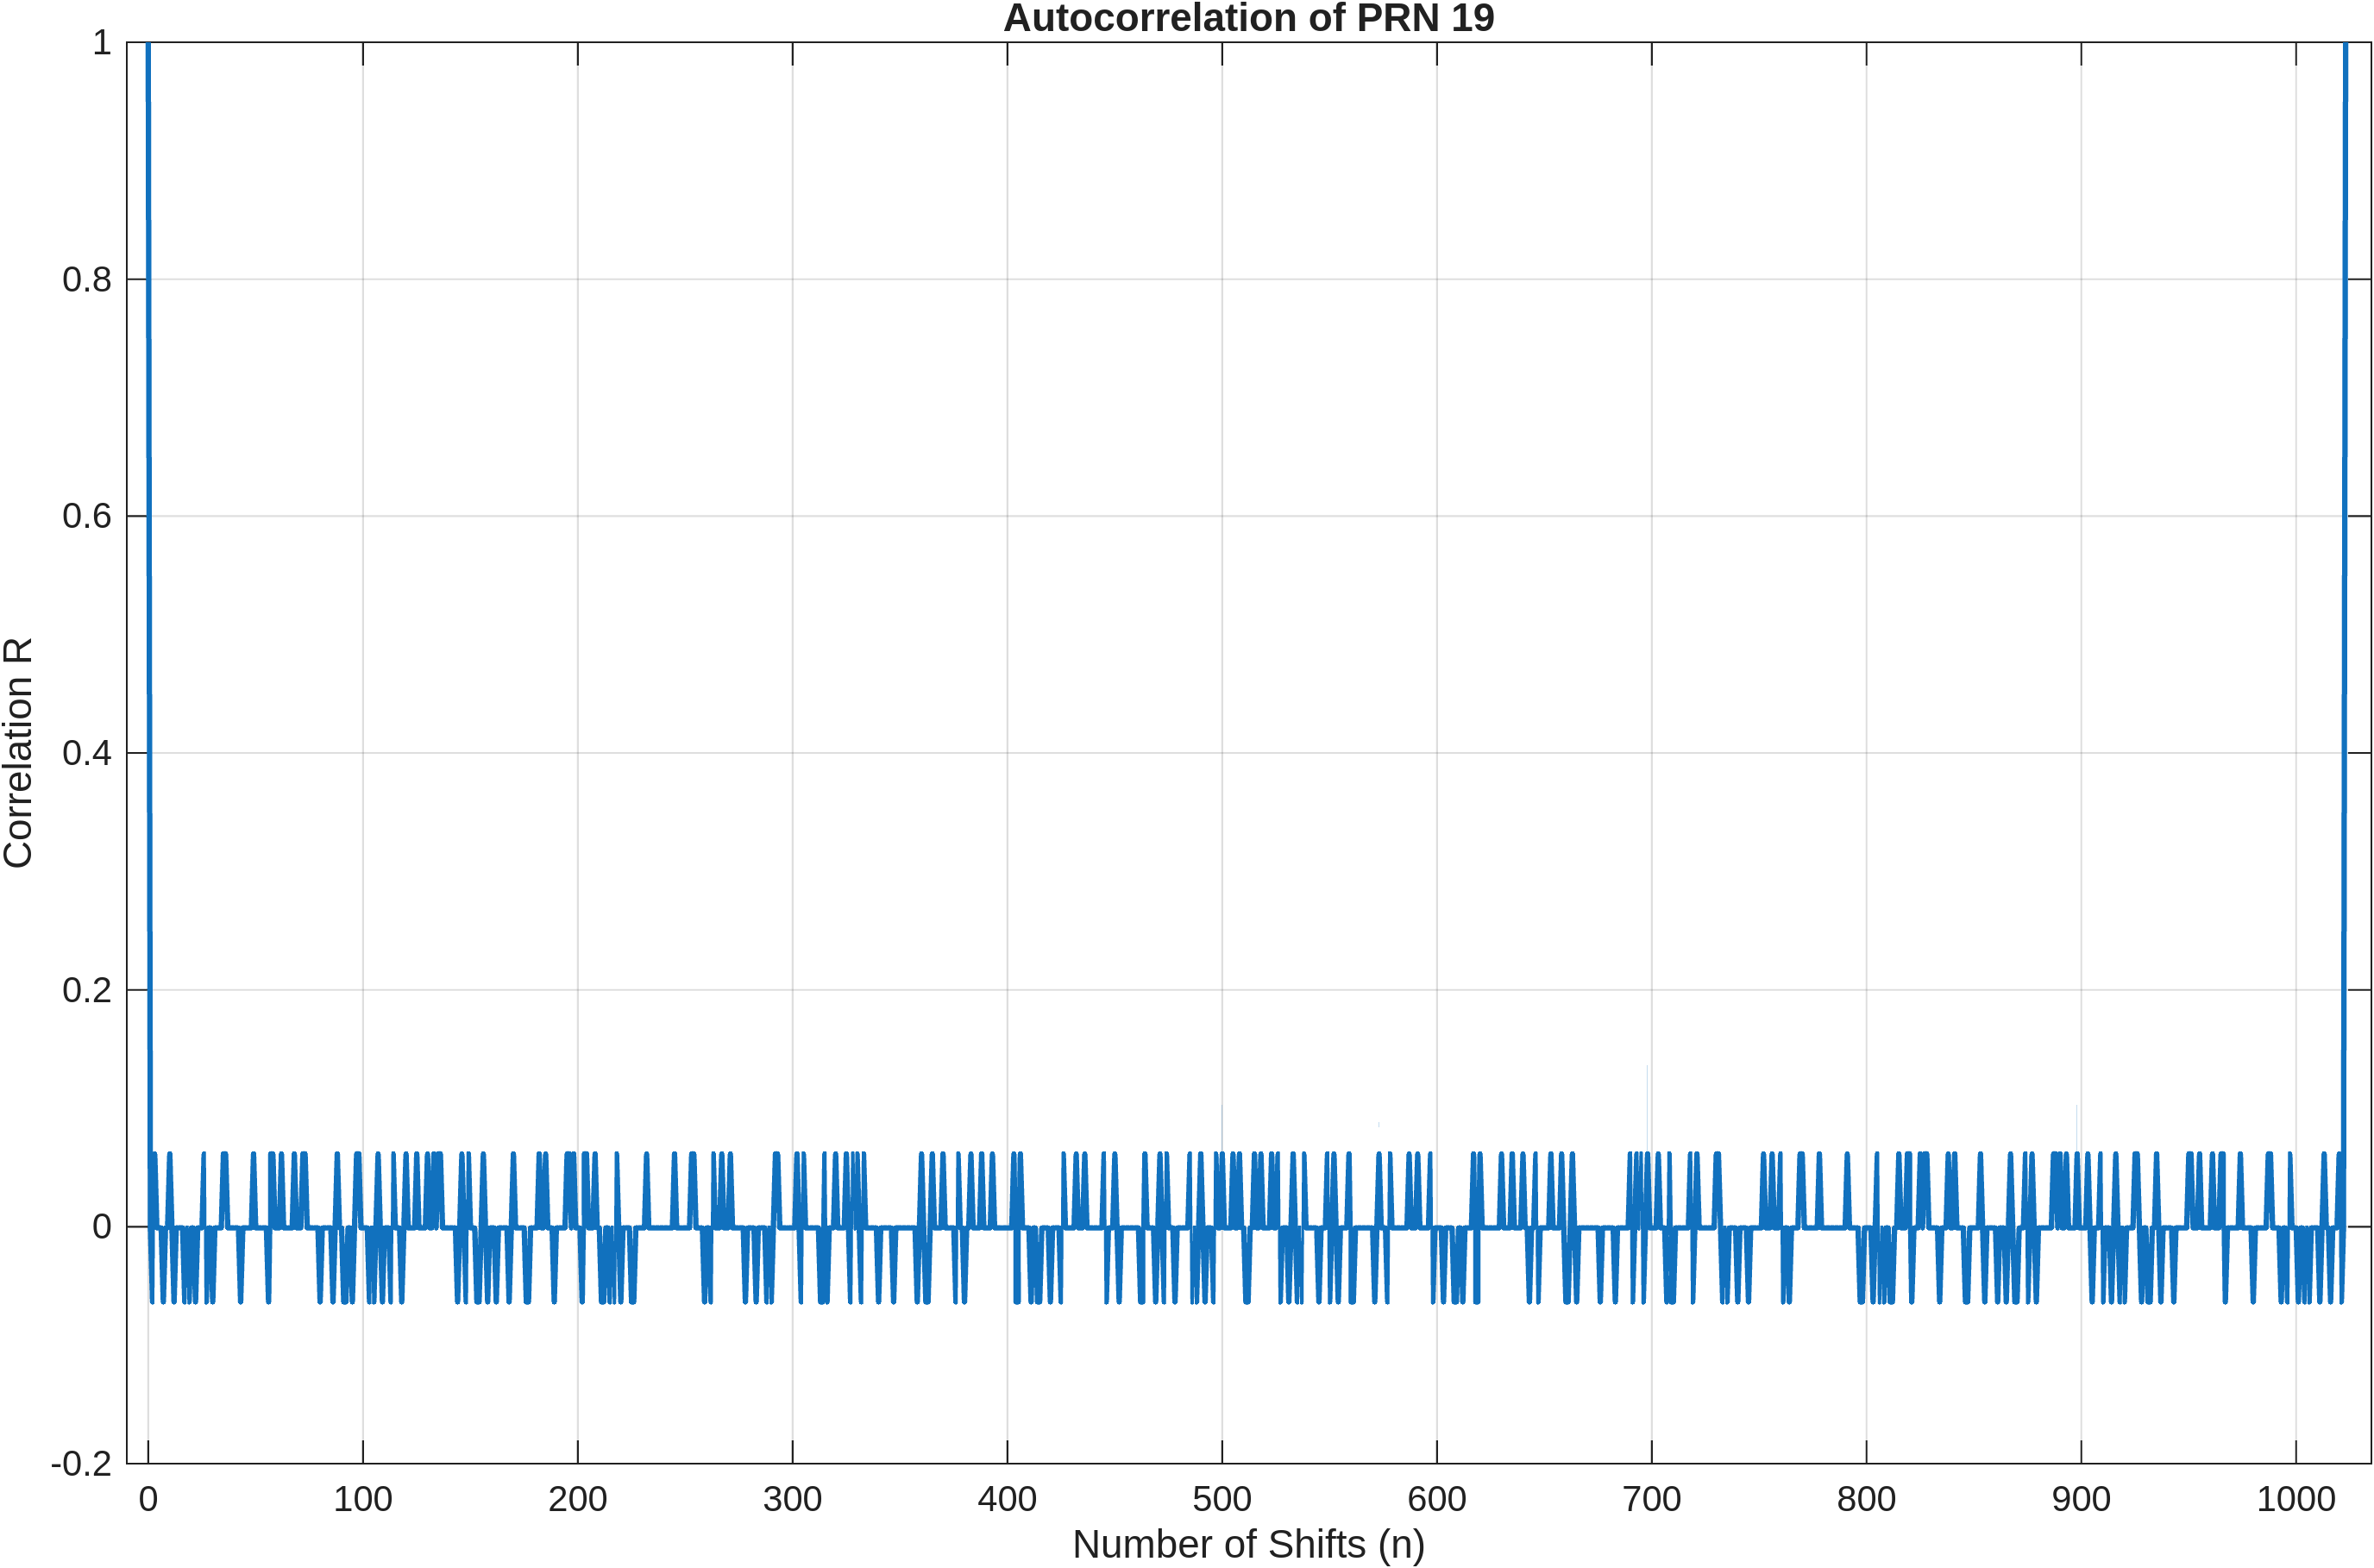
\includegraphics[width=0.8\textwidth]{../PRN19_Autocorrelation.png}
    \caption{PRN 19 Auto Correlation}
    \label{fig:PRN 19 Auto Correlation}
\end{figure}

\subsection*{(b.)}

\begin{figure}[H]
    \centering
    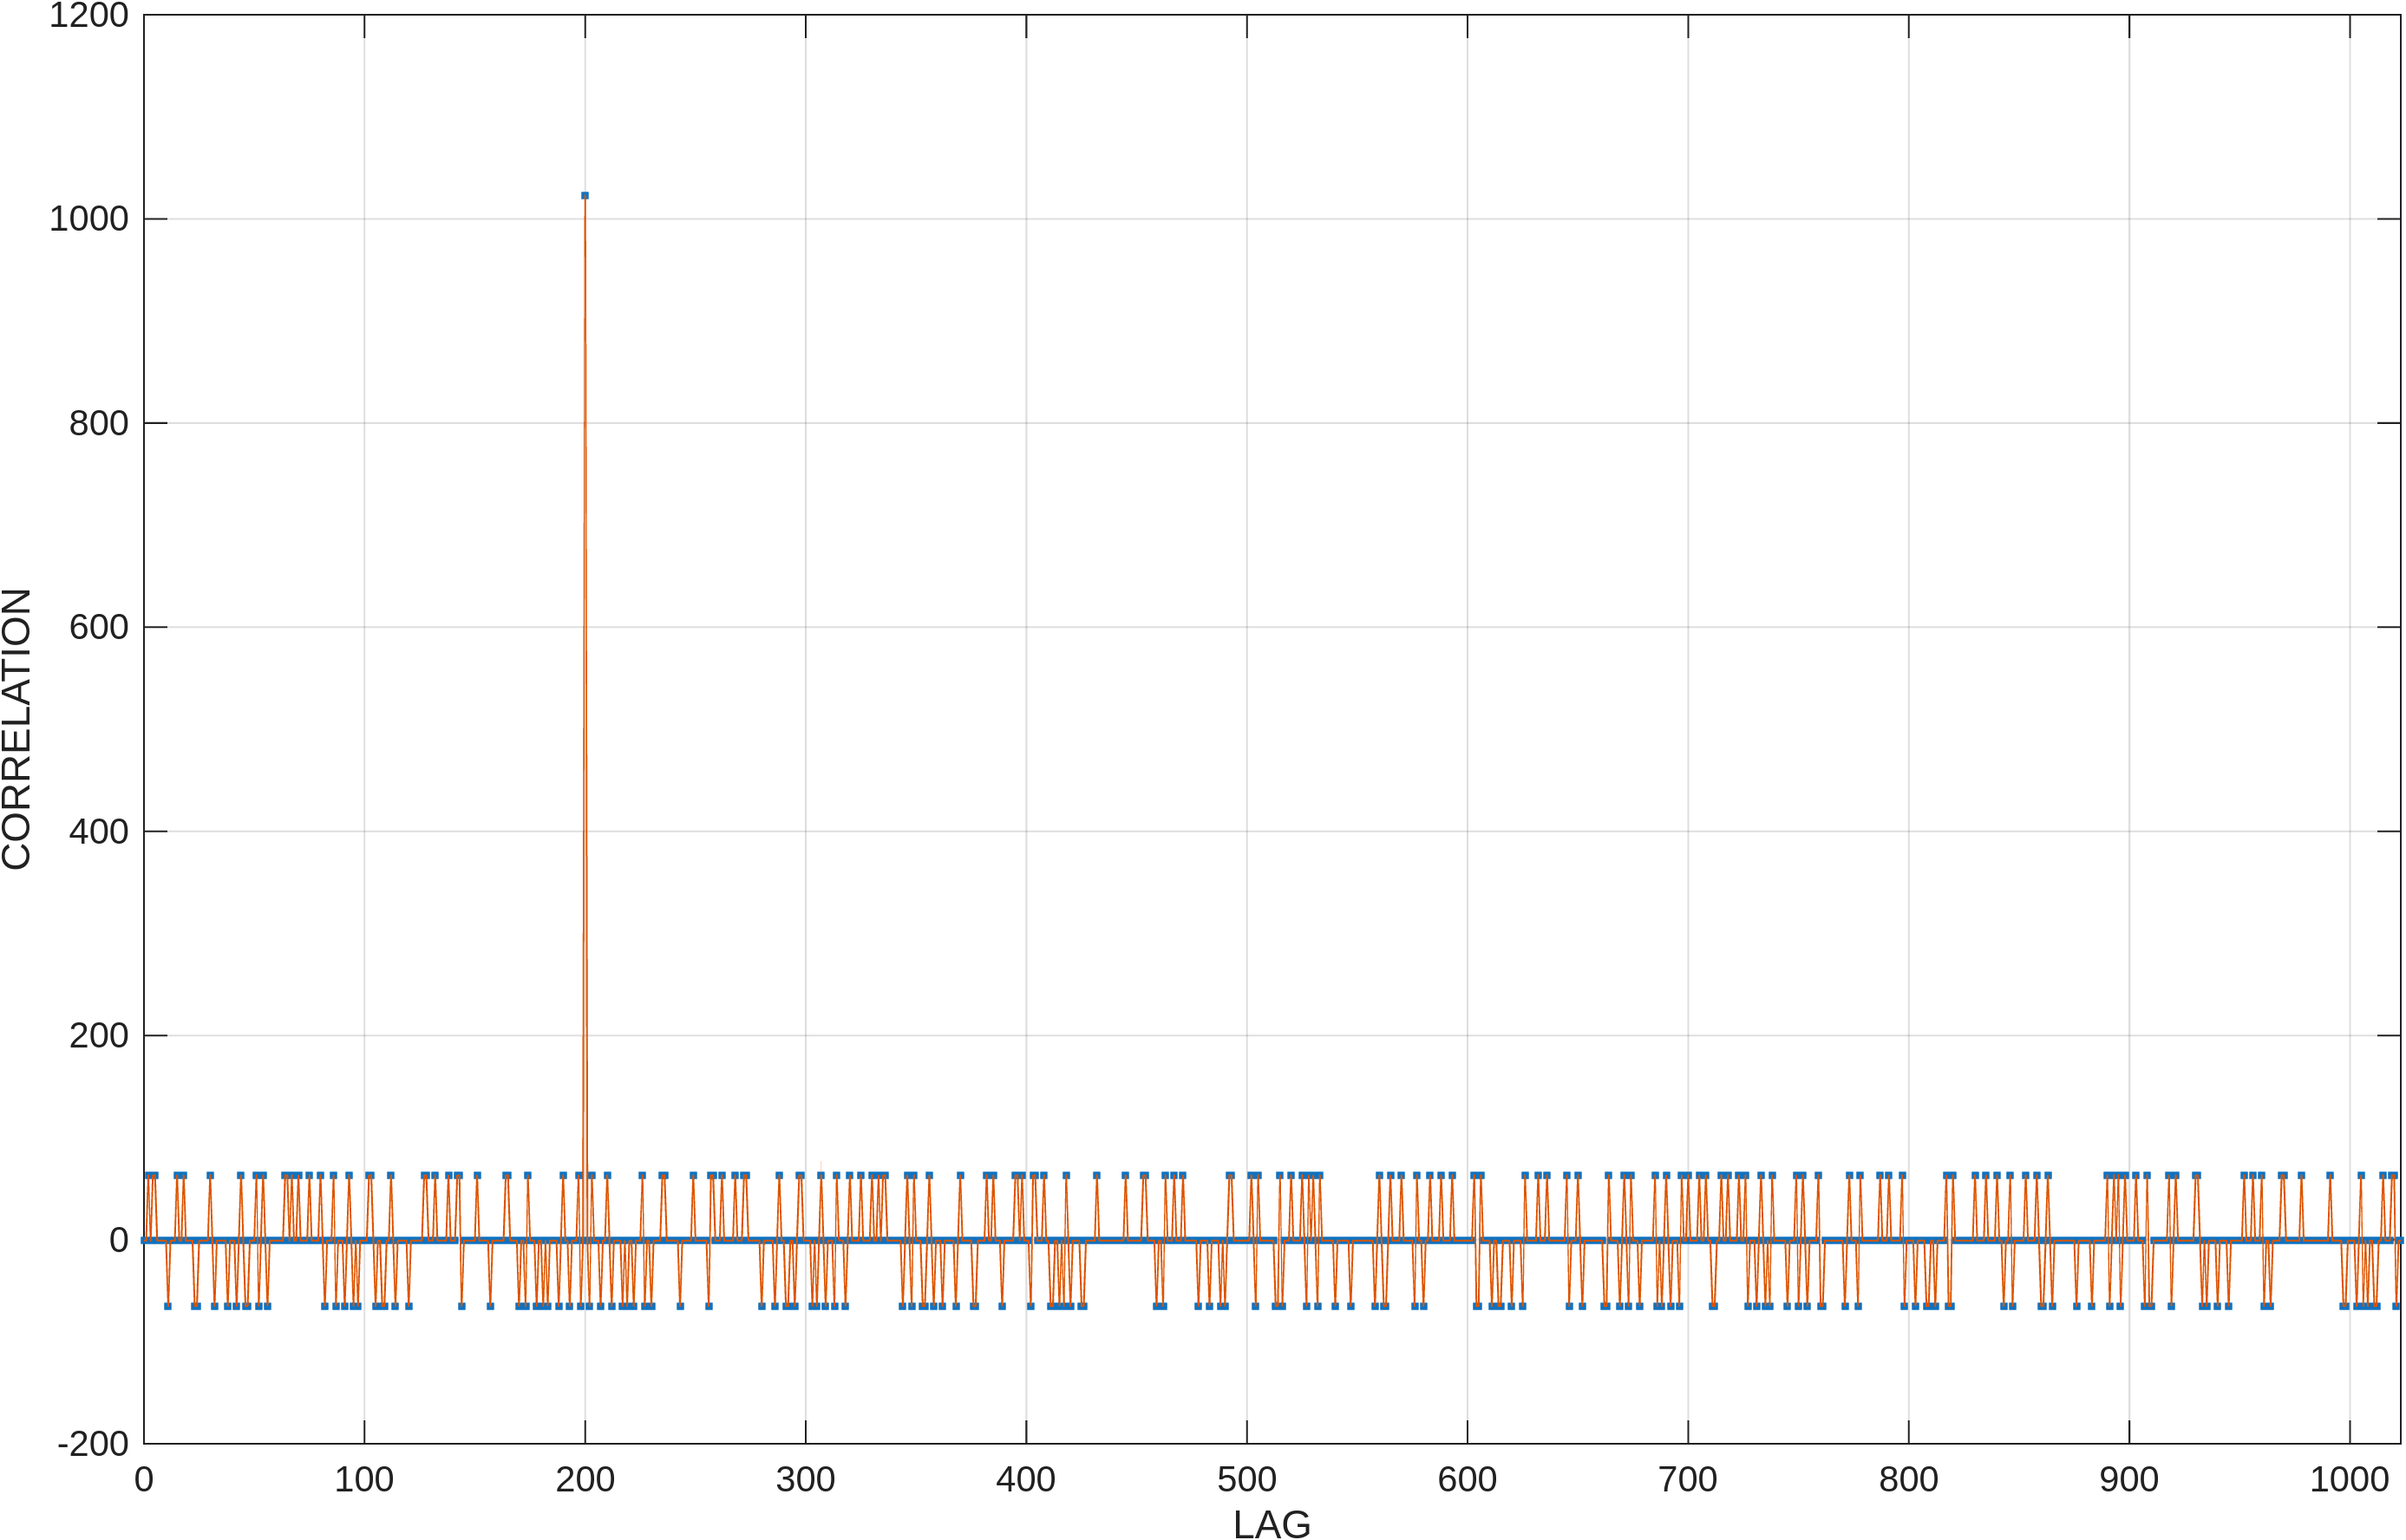
\includegraphics[width=0.8\textwidth]{../PRN19_PRN19_delay_200_Crosscorrelation.png}
    \caption{PRN 19 Delay Cross Correlation}
    \label{fig:PRN 19 Delay Cross Correlation}
\end{figure}

\hspace*{2em}Based on the Figure \ref{fig:PRN 19 Delay Cross Correlation}, results, we 
notice that there is a spike at 200 in the LAG axis. This is to be expected
since this function takes the cross correlation between two codes, because 
this is the same code only shifted, the spike occuring at the amount we shifted
it by is reasonable since at that point we would essentially be auto correlating 
the code resulting in similar behavior we observed in (a.). 

\subsection*{(c.)}

\begin{figure}[H]
    \centering
    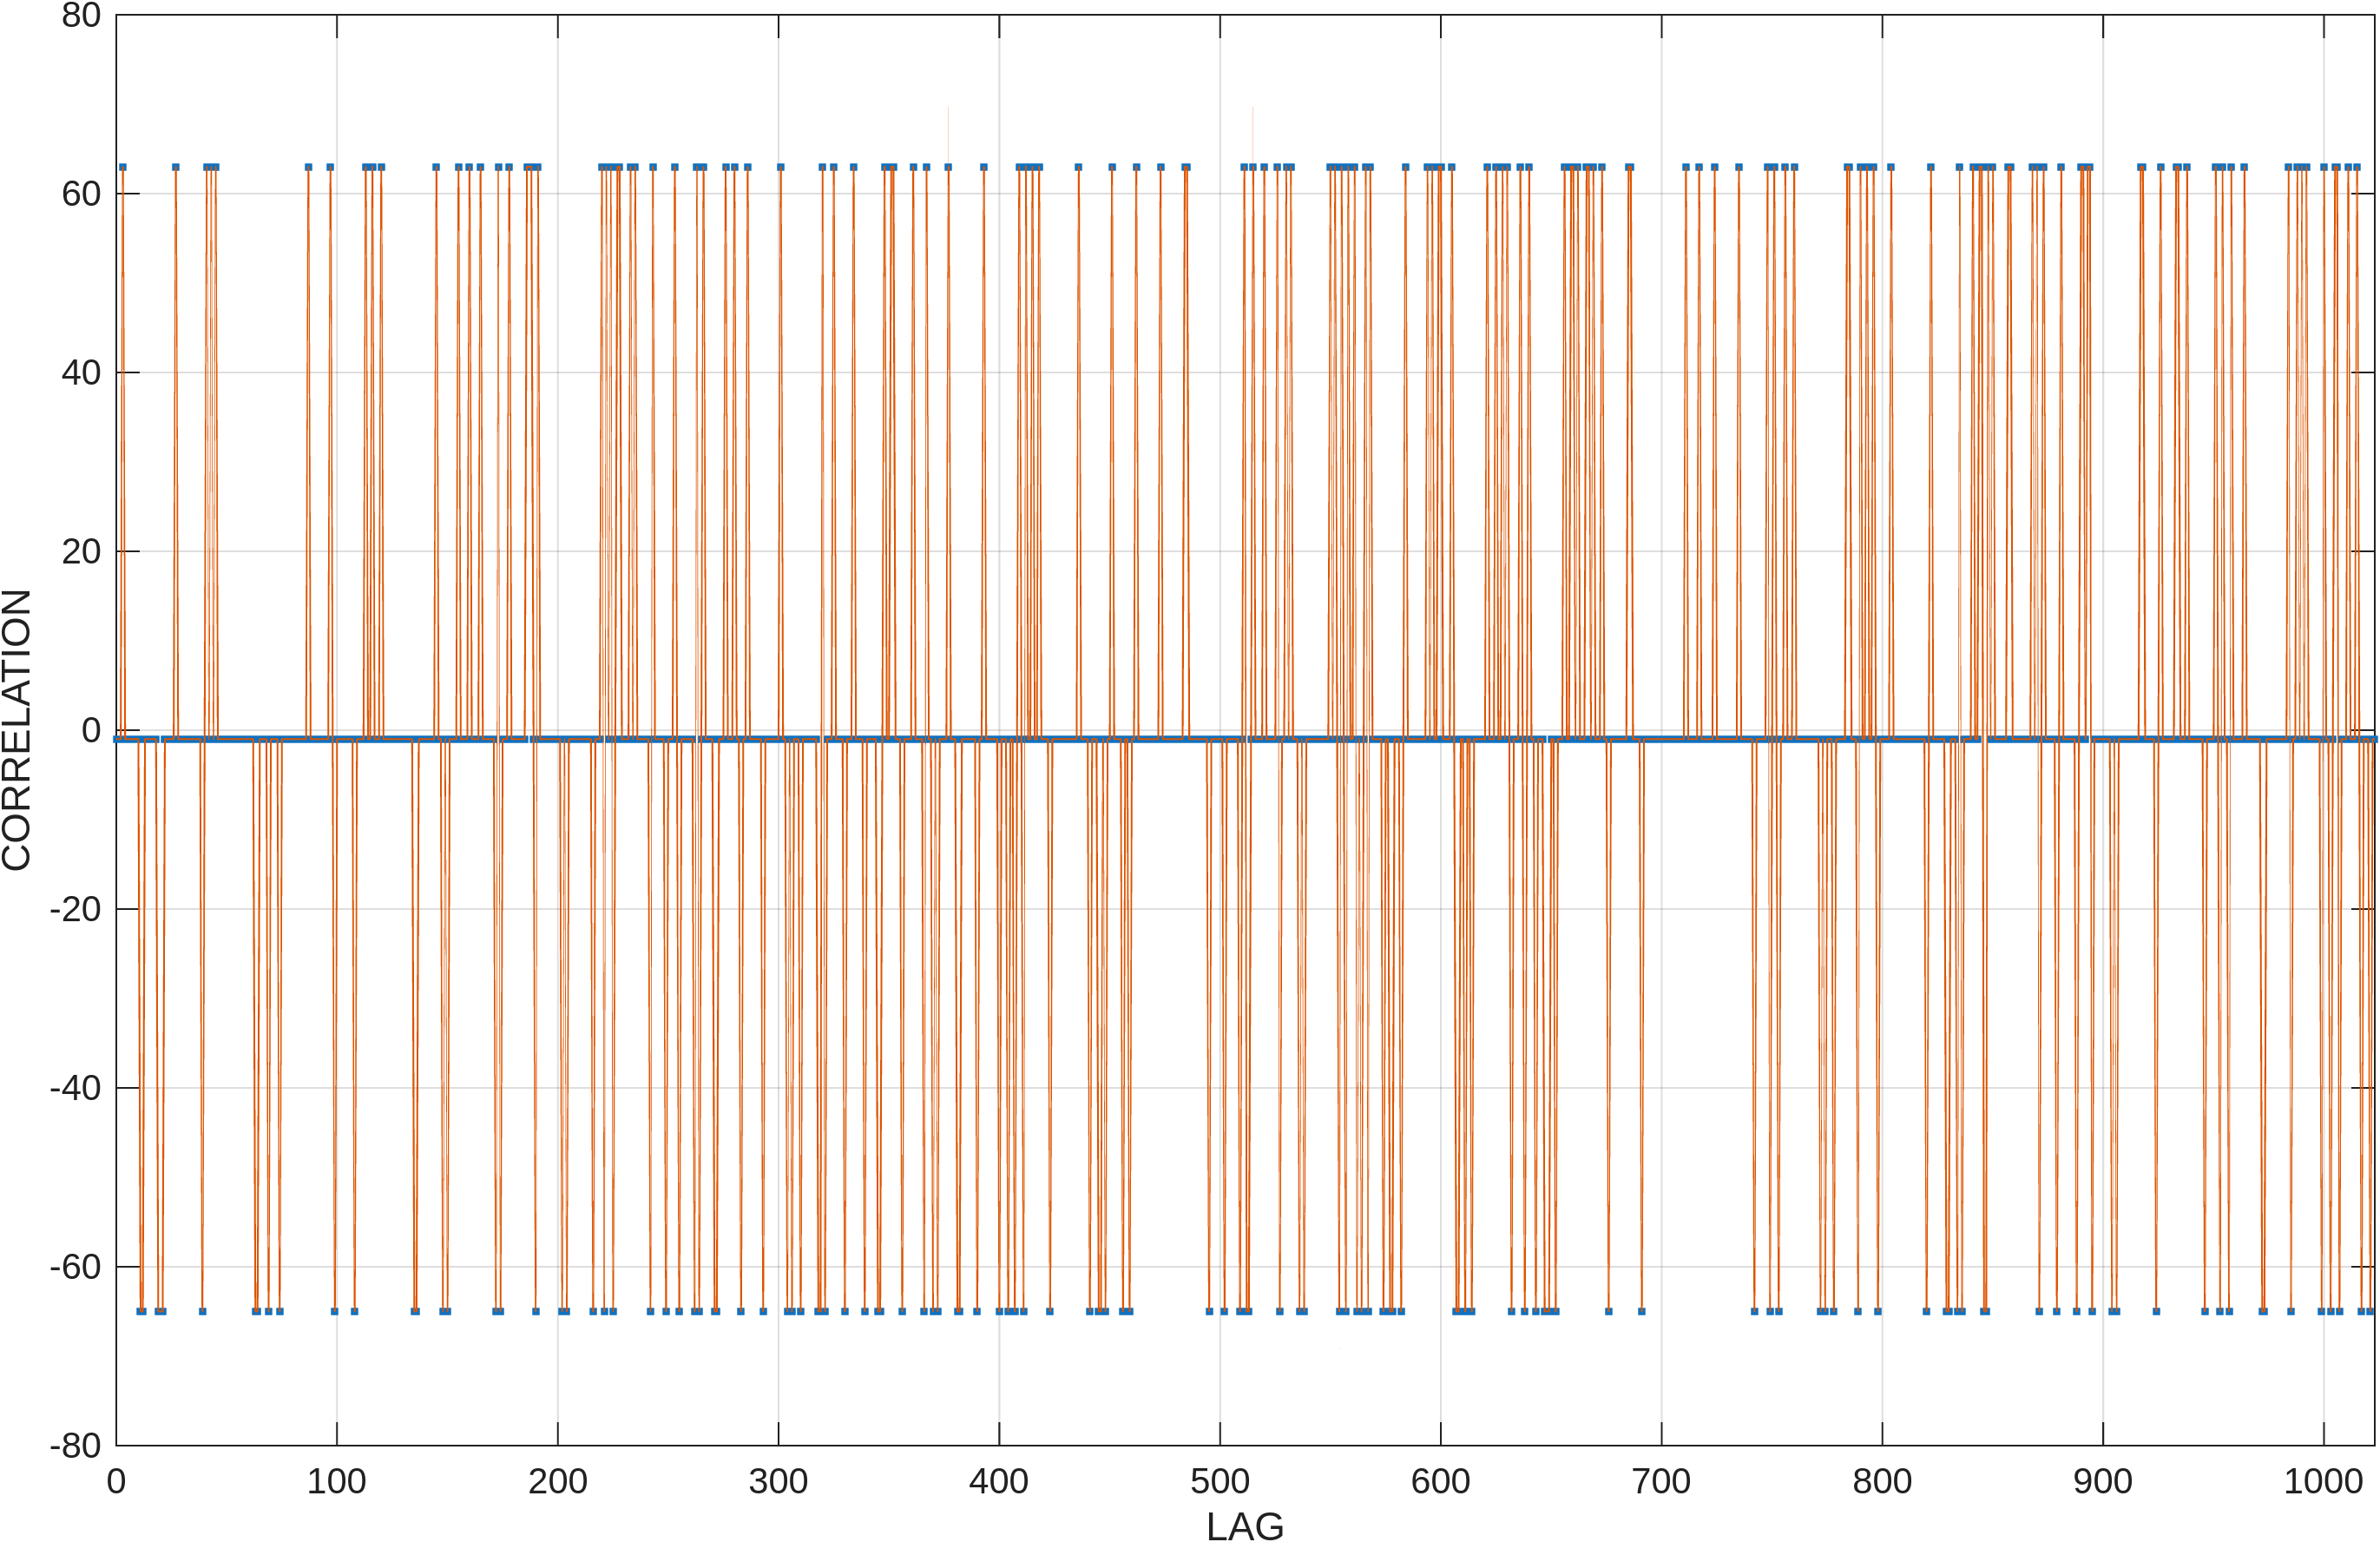
\includegraphics[width=0.8\textwidth]{../PRN25_PRN19_Crosscorrelation.png}
    \caption{PRN 25 Cross Correlation}
    \label{fig:PRN 25 Cross Correlation}
\end{figure}

\hspace*{2em}When comparing Figure \ref{fig:PRN 25 Cross Correlation} and the Figure \ref{fig:PRN 19 Auto Correlation}
from part (a.), we observe a different behavior. We see instead of a stable
variations of similar magnitude with a large spike where you would expect auto correlating
behavior, there is instead only a stable variation of similar magnitude with no spike.

\subsection*{(d.)}

\begin{figure}[H]
    \centering
    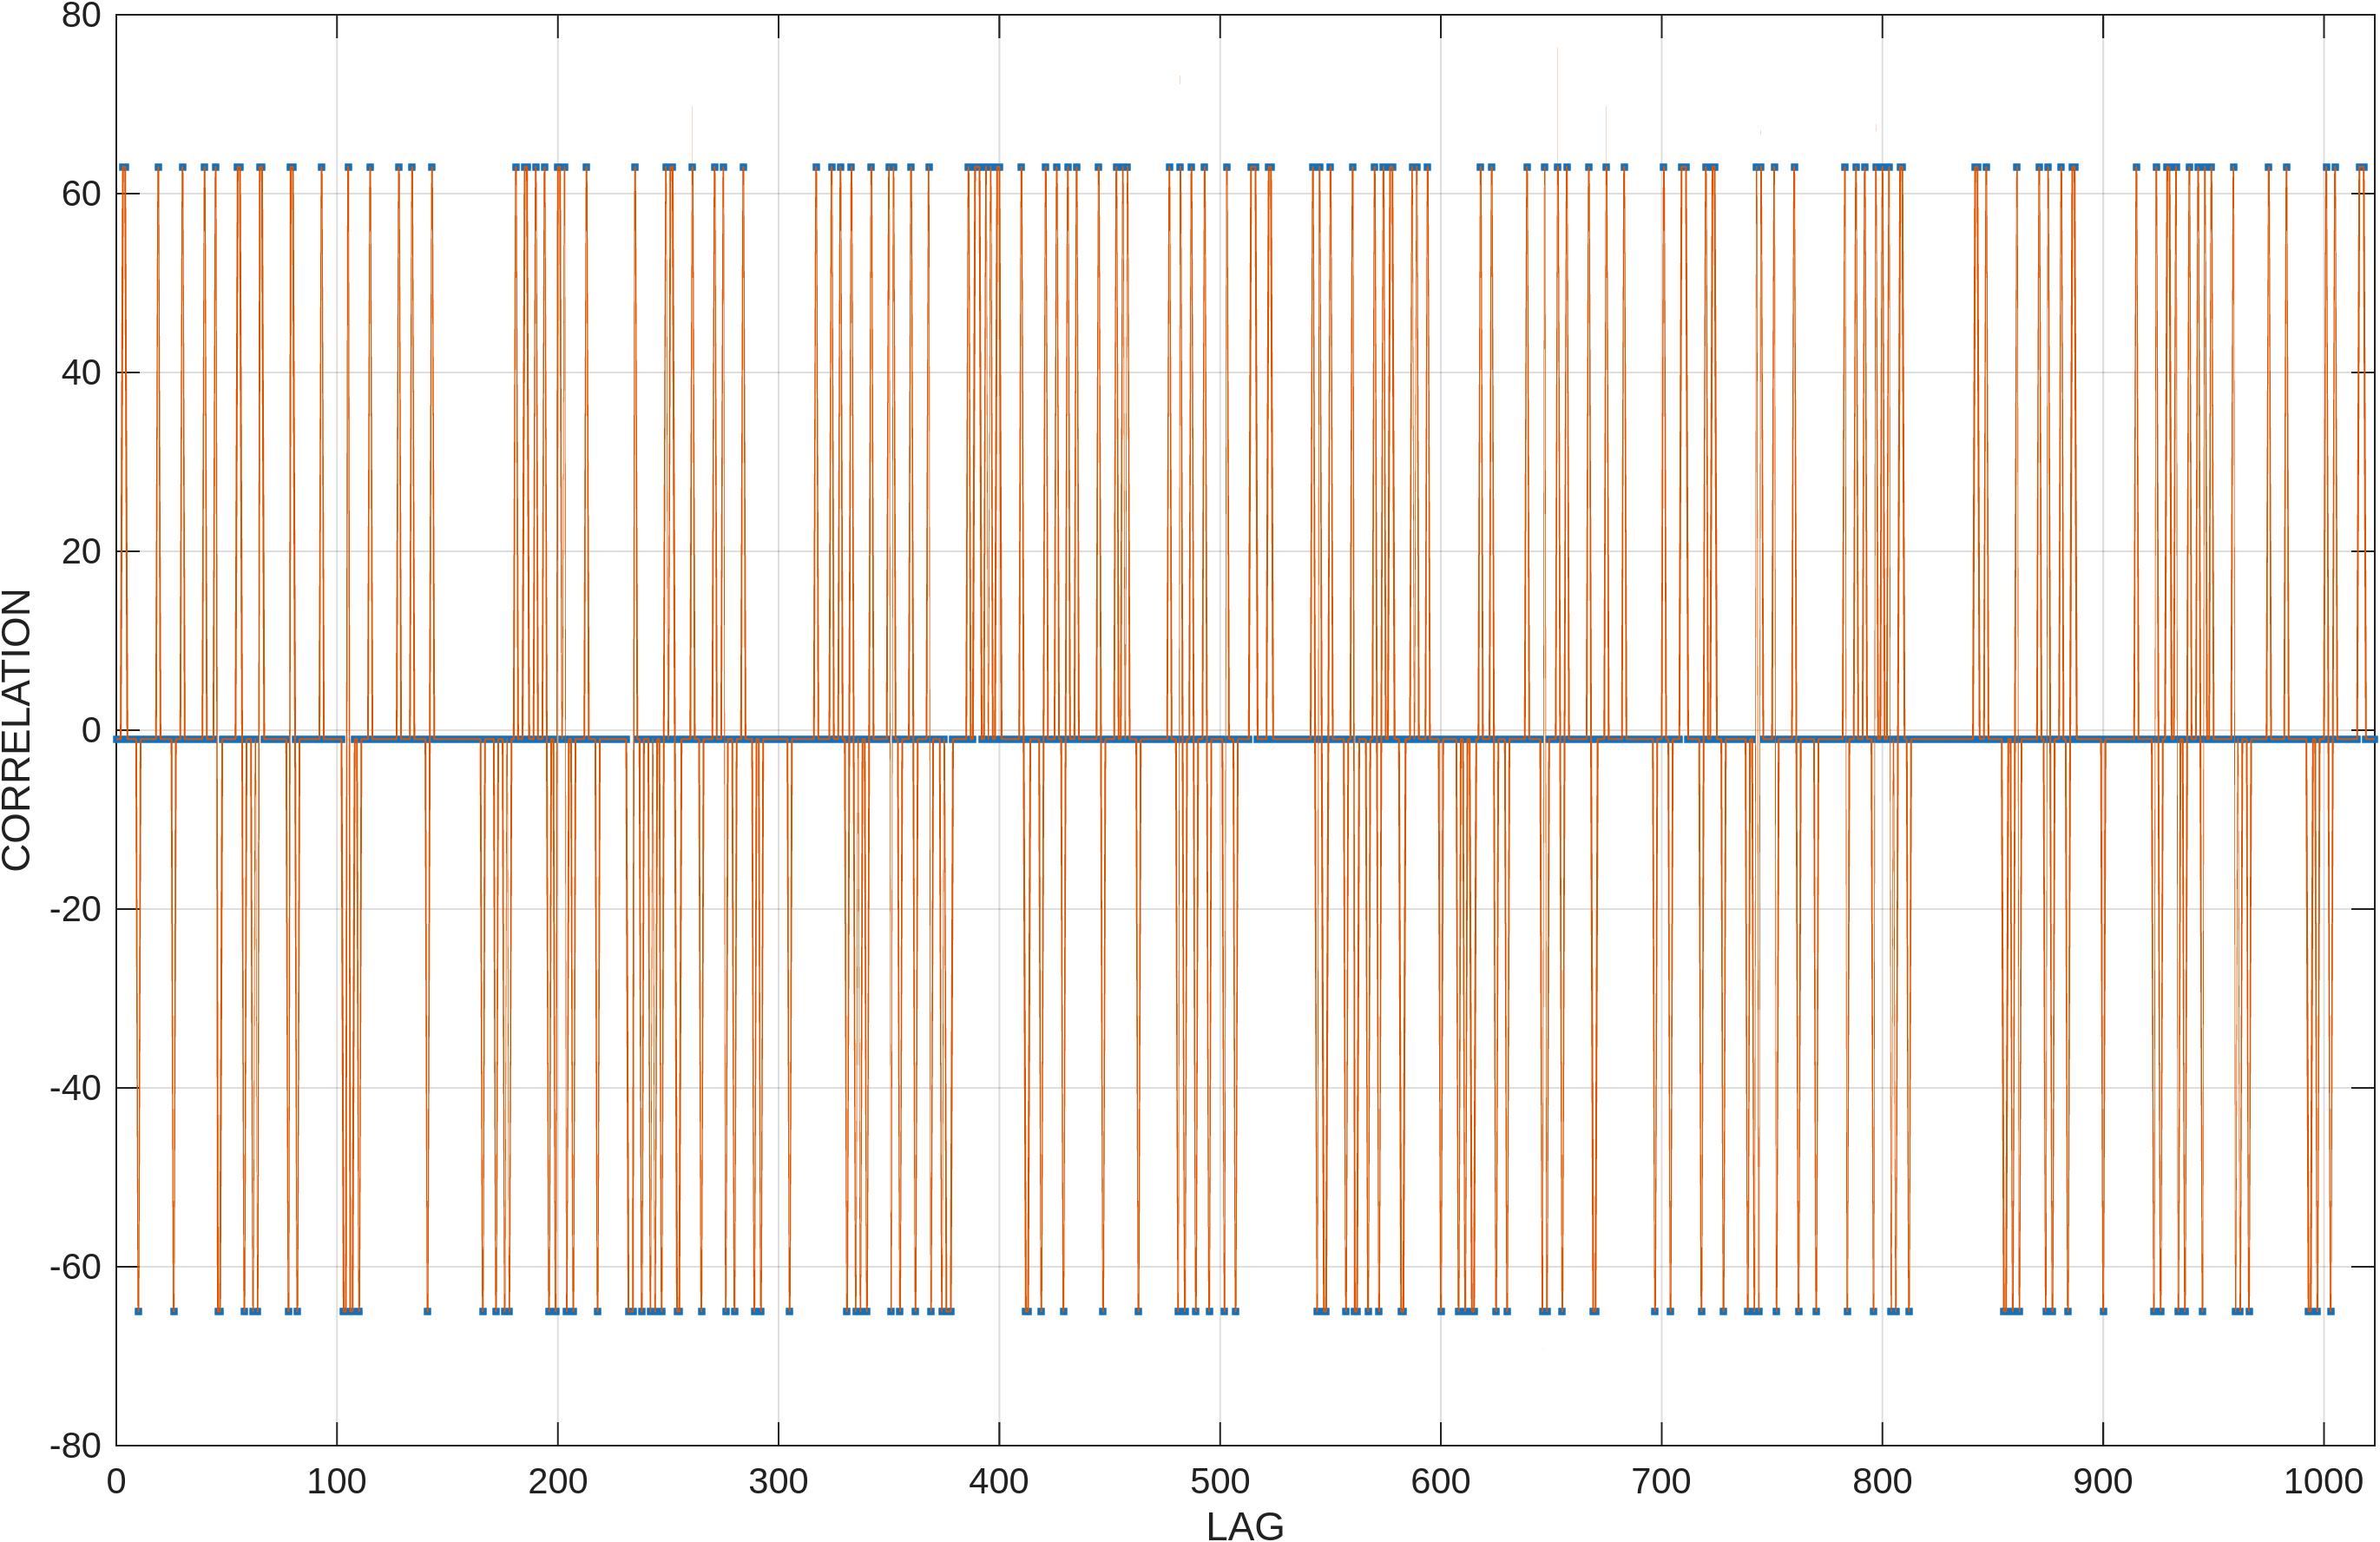
\includegraphics[width=0.8\textwidth]{../PRN5_PRN19_Crosscorrelation.png}
    \caption{PRN 5 Cross Correlation}
    \label{fig:PRN 5 Cross Correlation}
\end{figure}

\hspace*{2em}Similarly when comparing Figure \ref{fig:PRN 5 Cross Correlation} with Figure \ref{fig:PRN 19 Auto Correlation}
from part (a)., we observe similar variations as we observed in part (c.). Where 
it is missing a spike and only has variations of similar magnitude.

\subsection*{(e.)}

\begin{figure}[H]
    \centering
    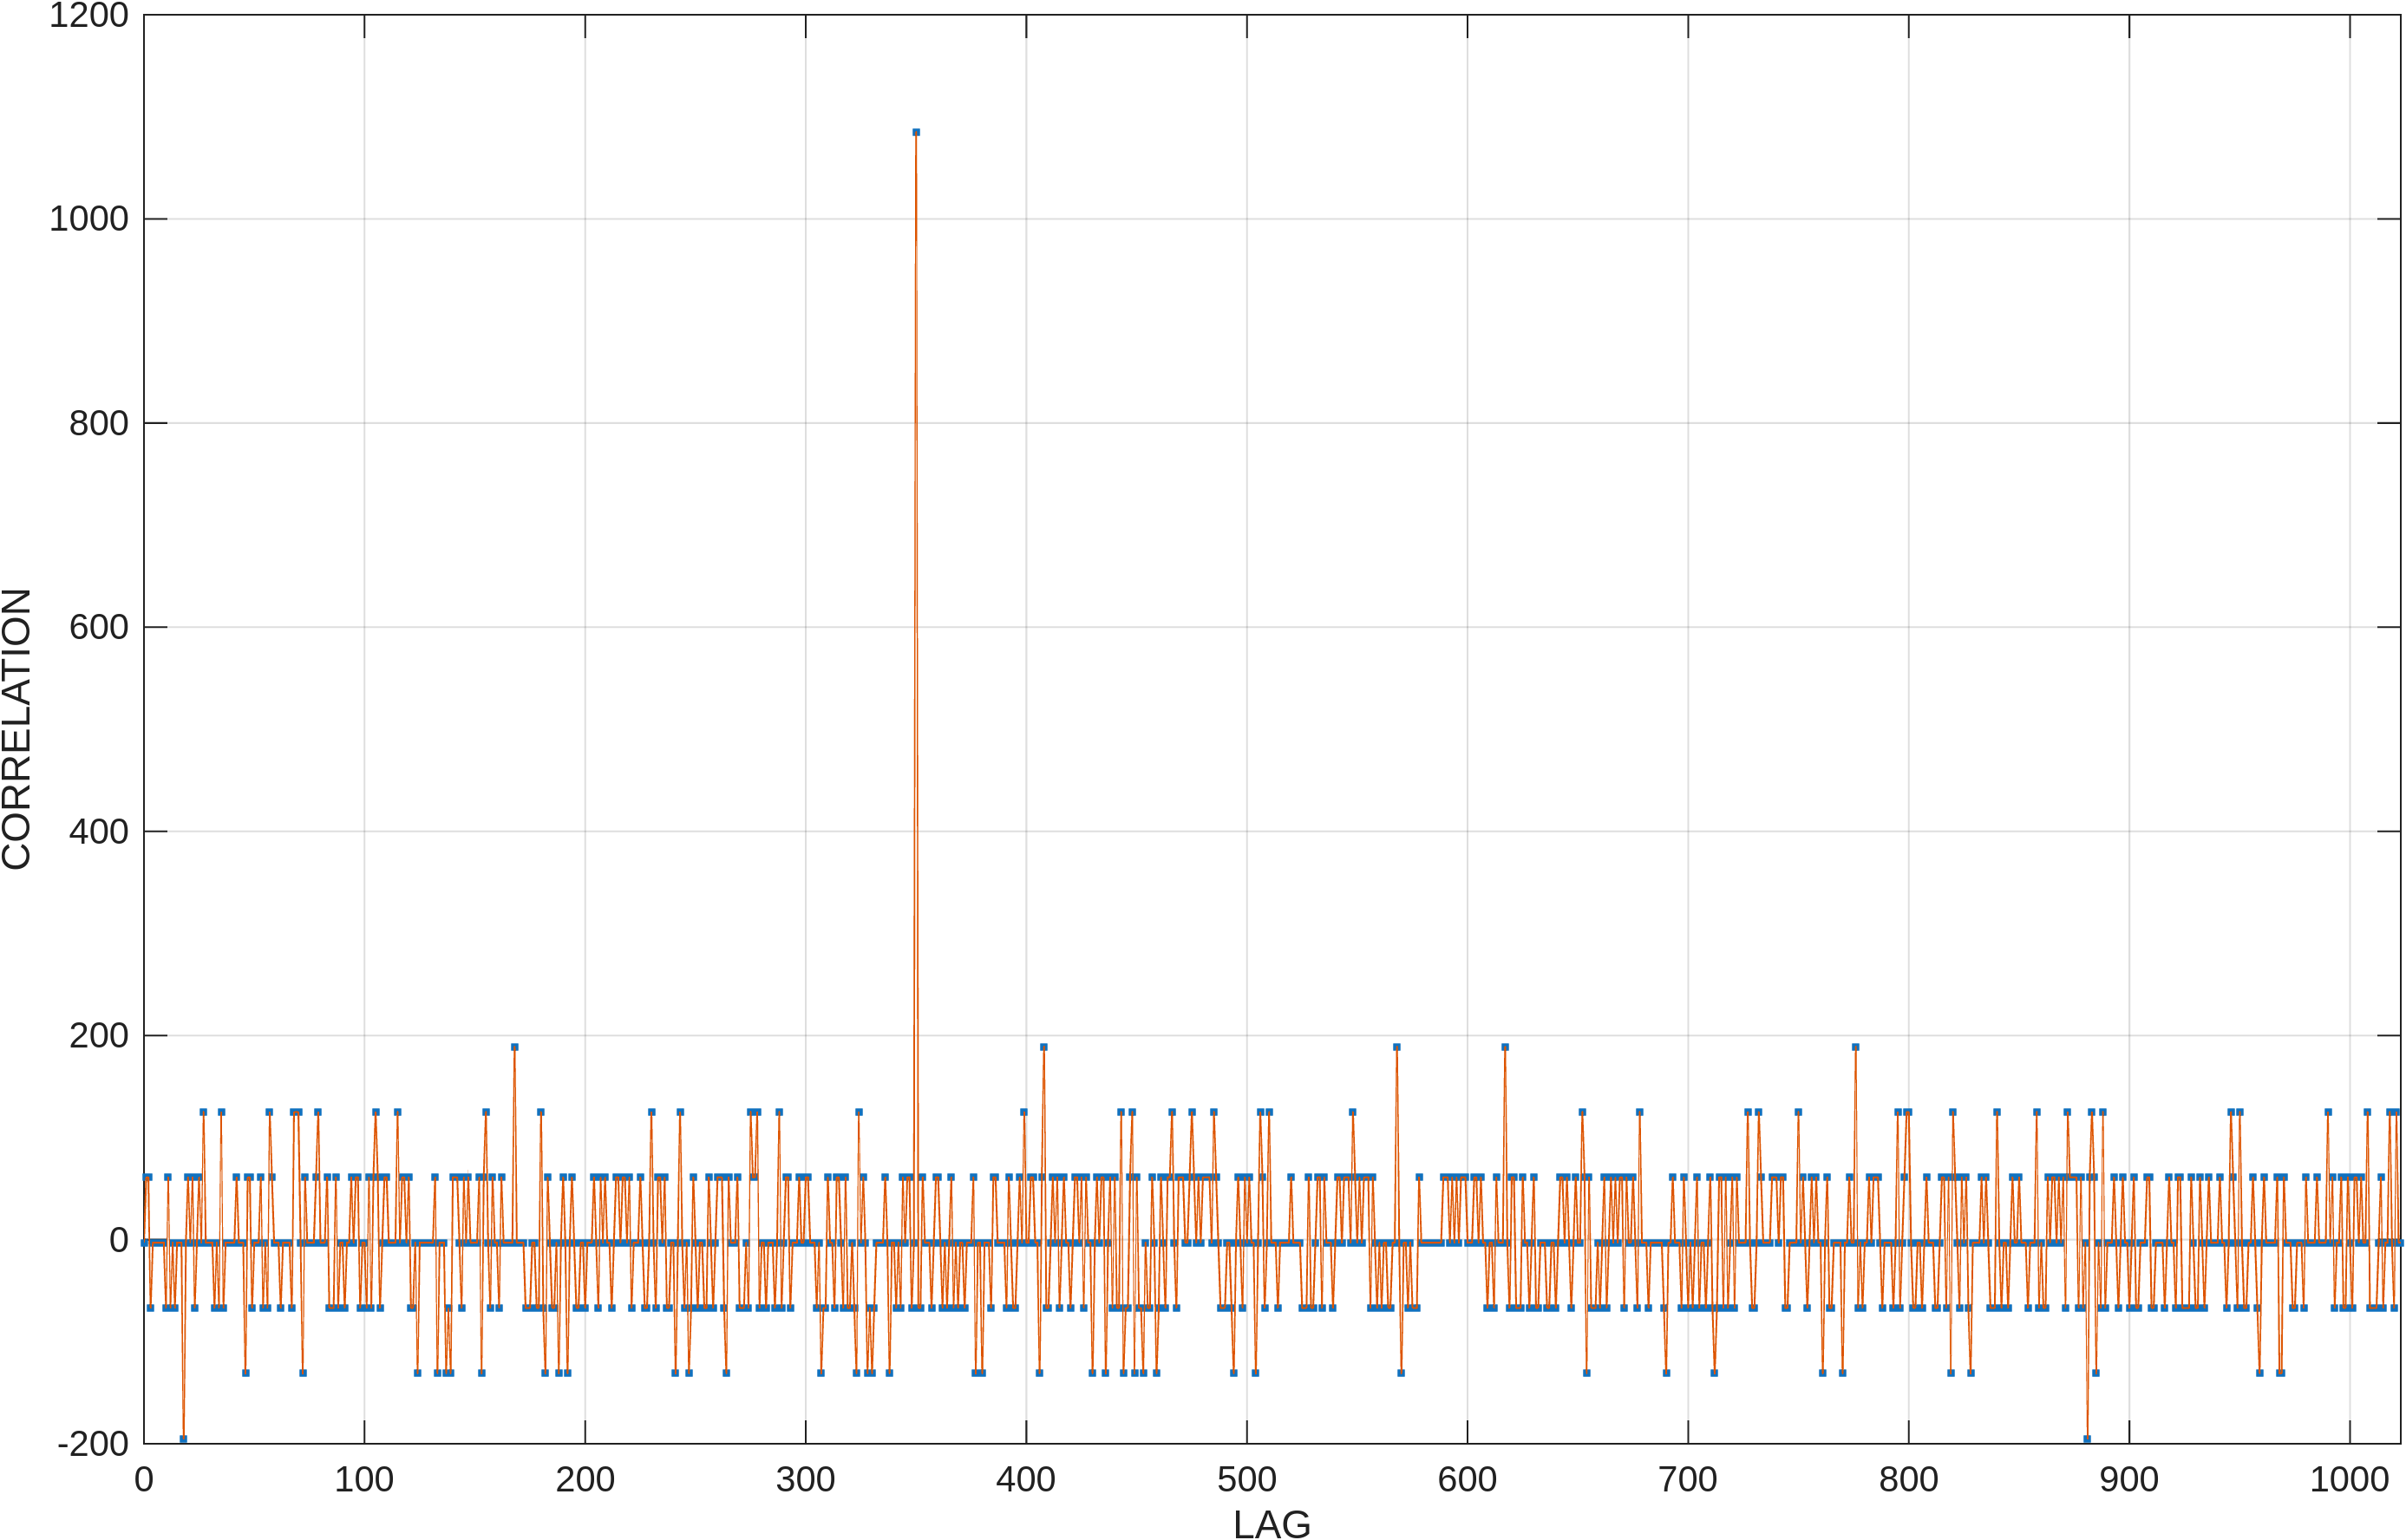
\includegraphics[width=0.8\textwidth]{../PRN5xsum_PRN19_Crosscorrelation.png}
    \caption{PRN Cross Correlation of sum of $x1,x2,x3$}
    \label{fig:PRN xsum cross correlation}
\end{figure}

\hspace*{2em}The peak of the correlation within Figure \ref{fig:PRN xsum cross correlation} is 
indeed where I would expect it to be. Essentially we are mixing together multiple competing
PRN signals from a GPS satellite. Because of how these codes are constructued, these codes
have high auto correlation and low cross correlation with each other. Therefore, when these
signals are mixed together and cross correlate with PRN 19, PRN 19 will have a spike where 
it would auto correlate to the respective chip shift on the lag axis, which in this 
case is 350. 

\subsection*{(f.)}

\begin{figure}[H]
    \centering
    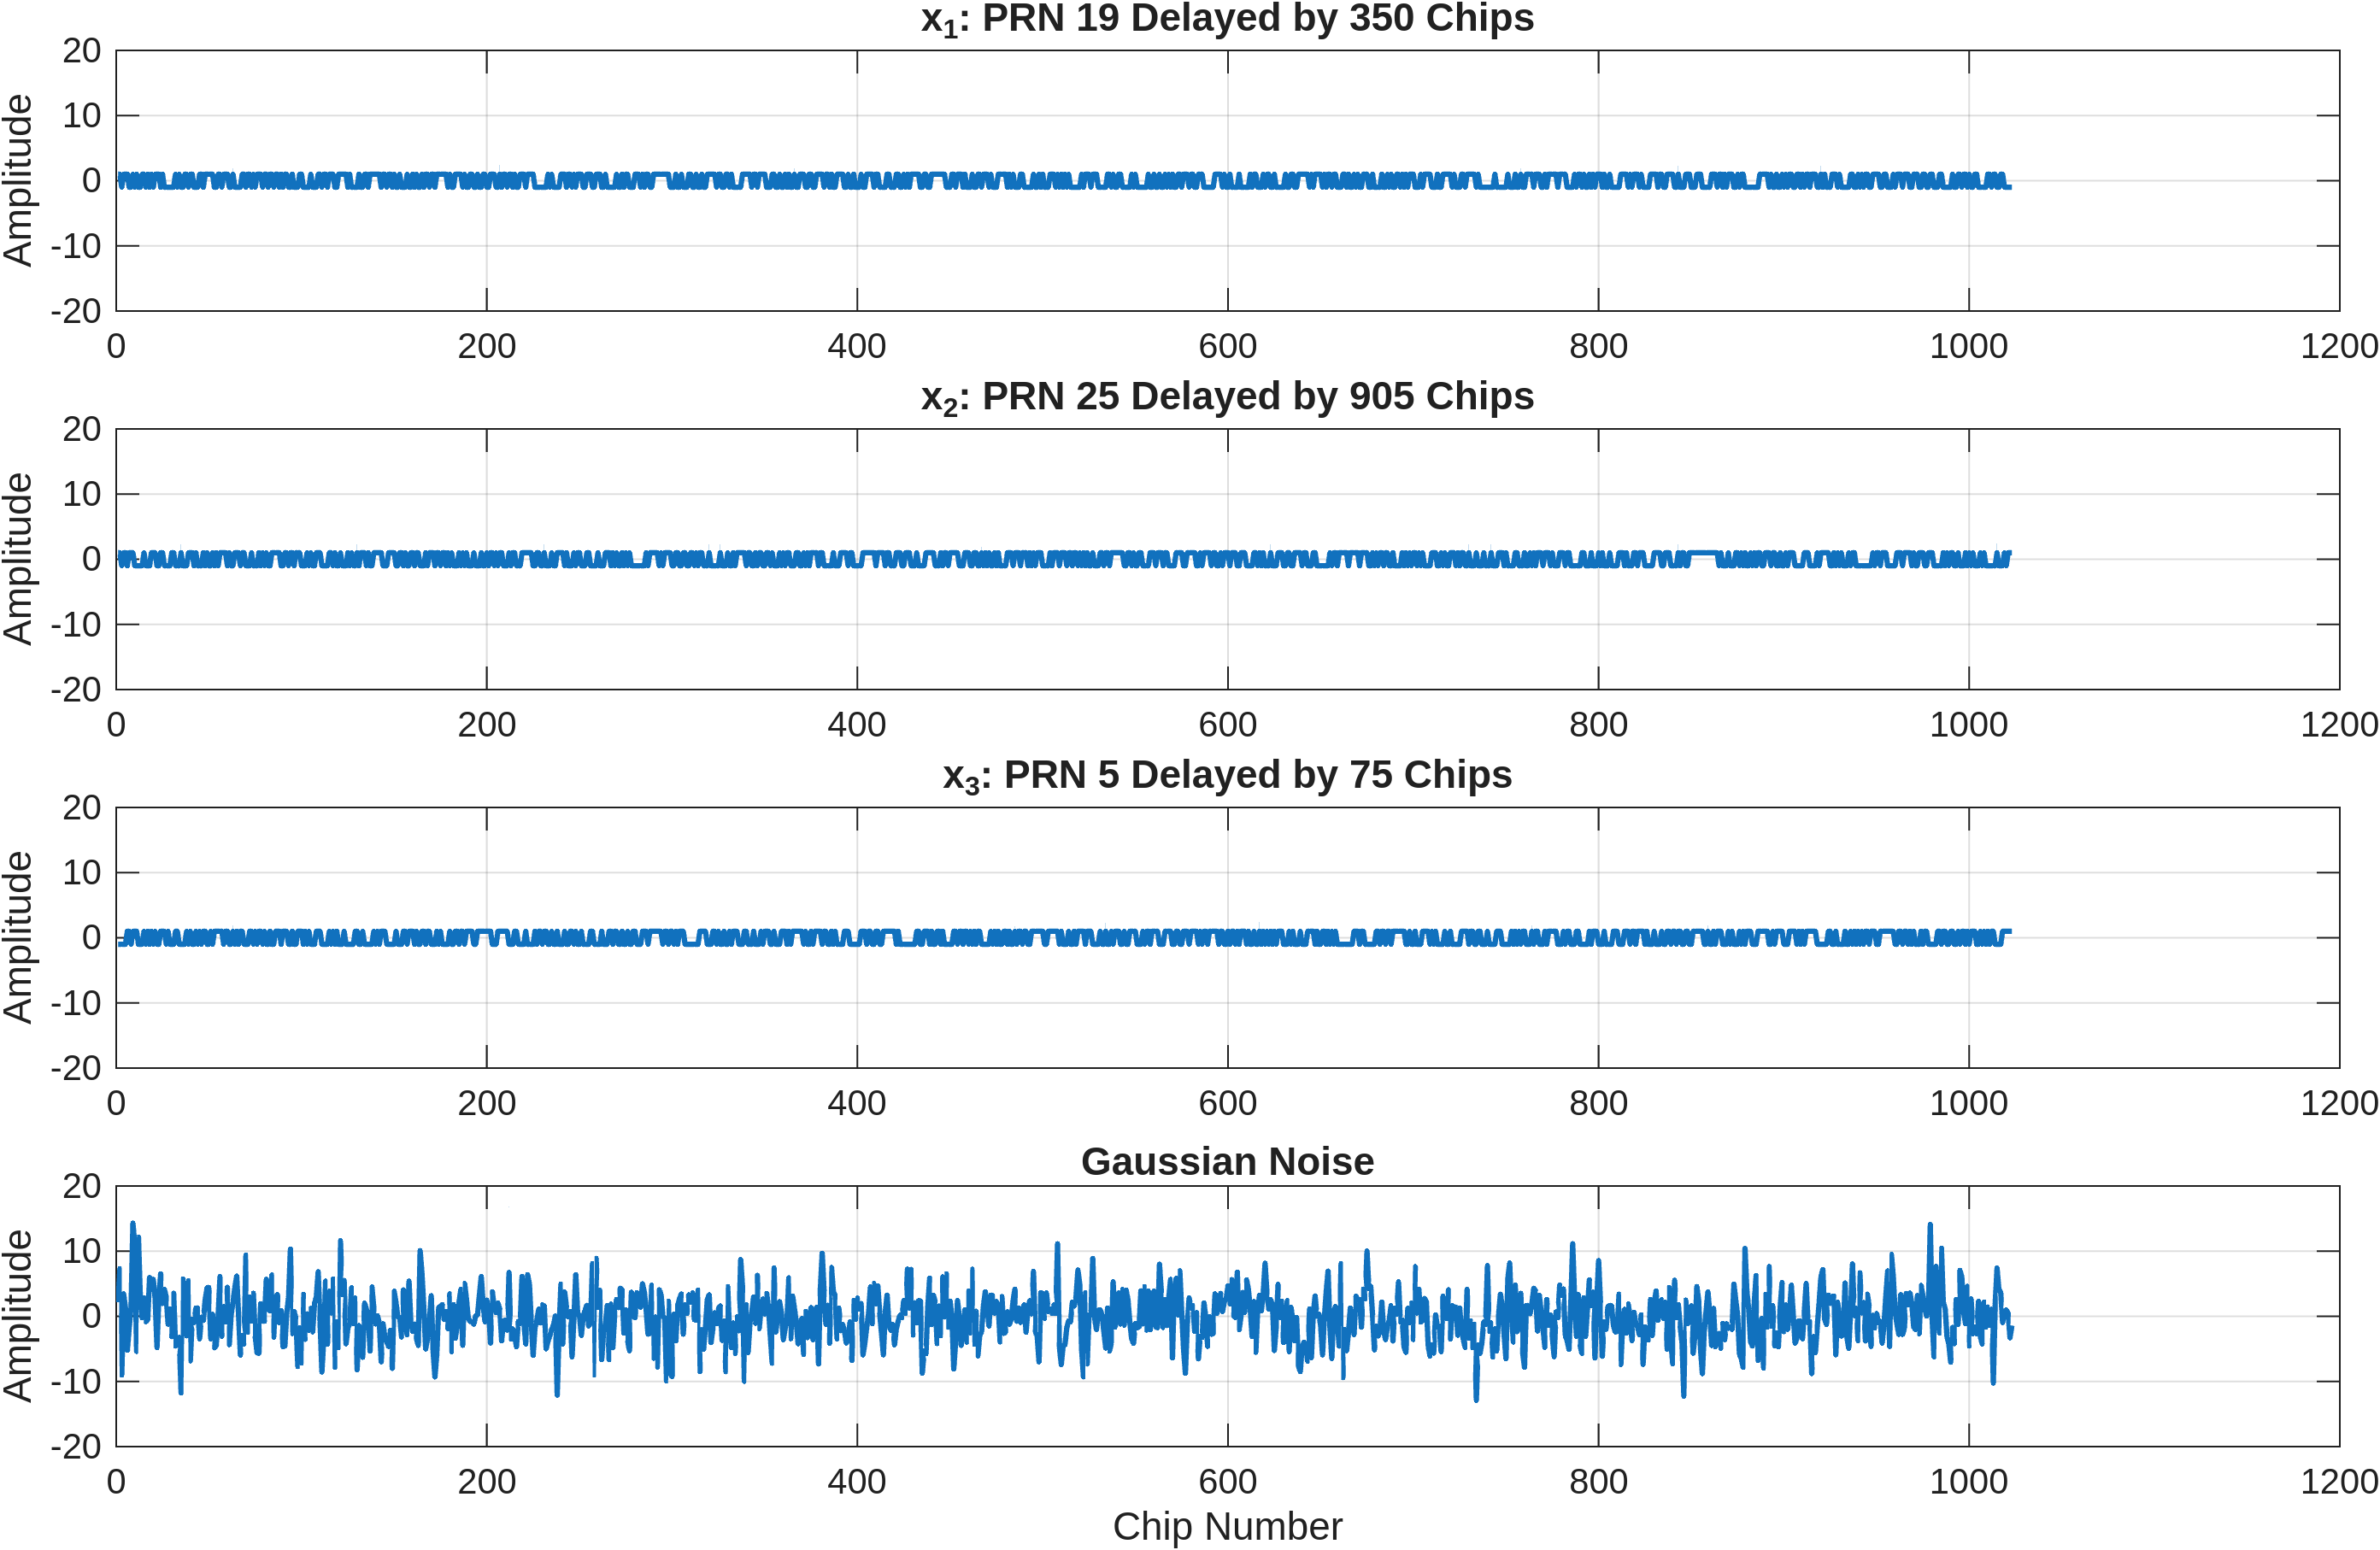
\includegraphics[width=0.8\textwidth]{../subplot_x1x2x3_noise.png}
    \caption{PRN Cross Correlation of sum of $x_1,x_2,x_3$}
    \label{fig:x1x2x3_noise_plot}
\end{figure}

\subsection*{(g.)}
\begin{figure}[H]
    \centering
    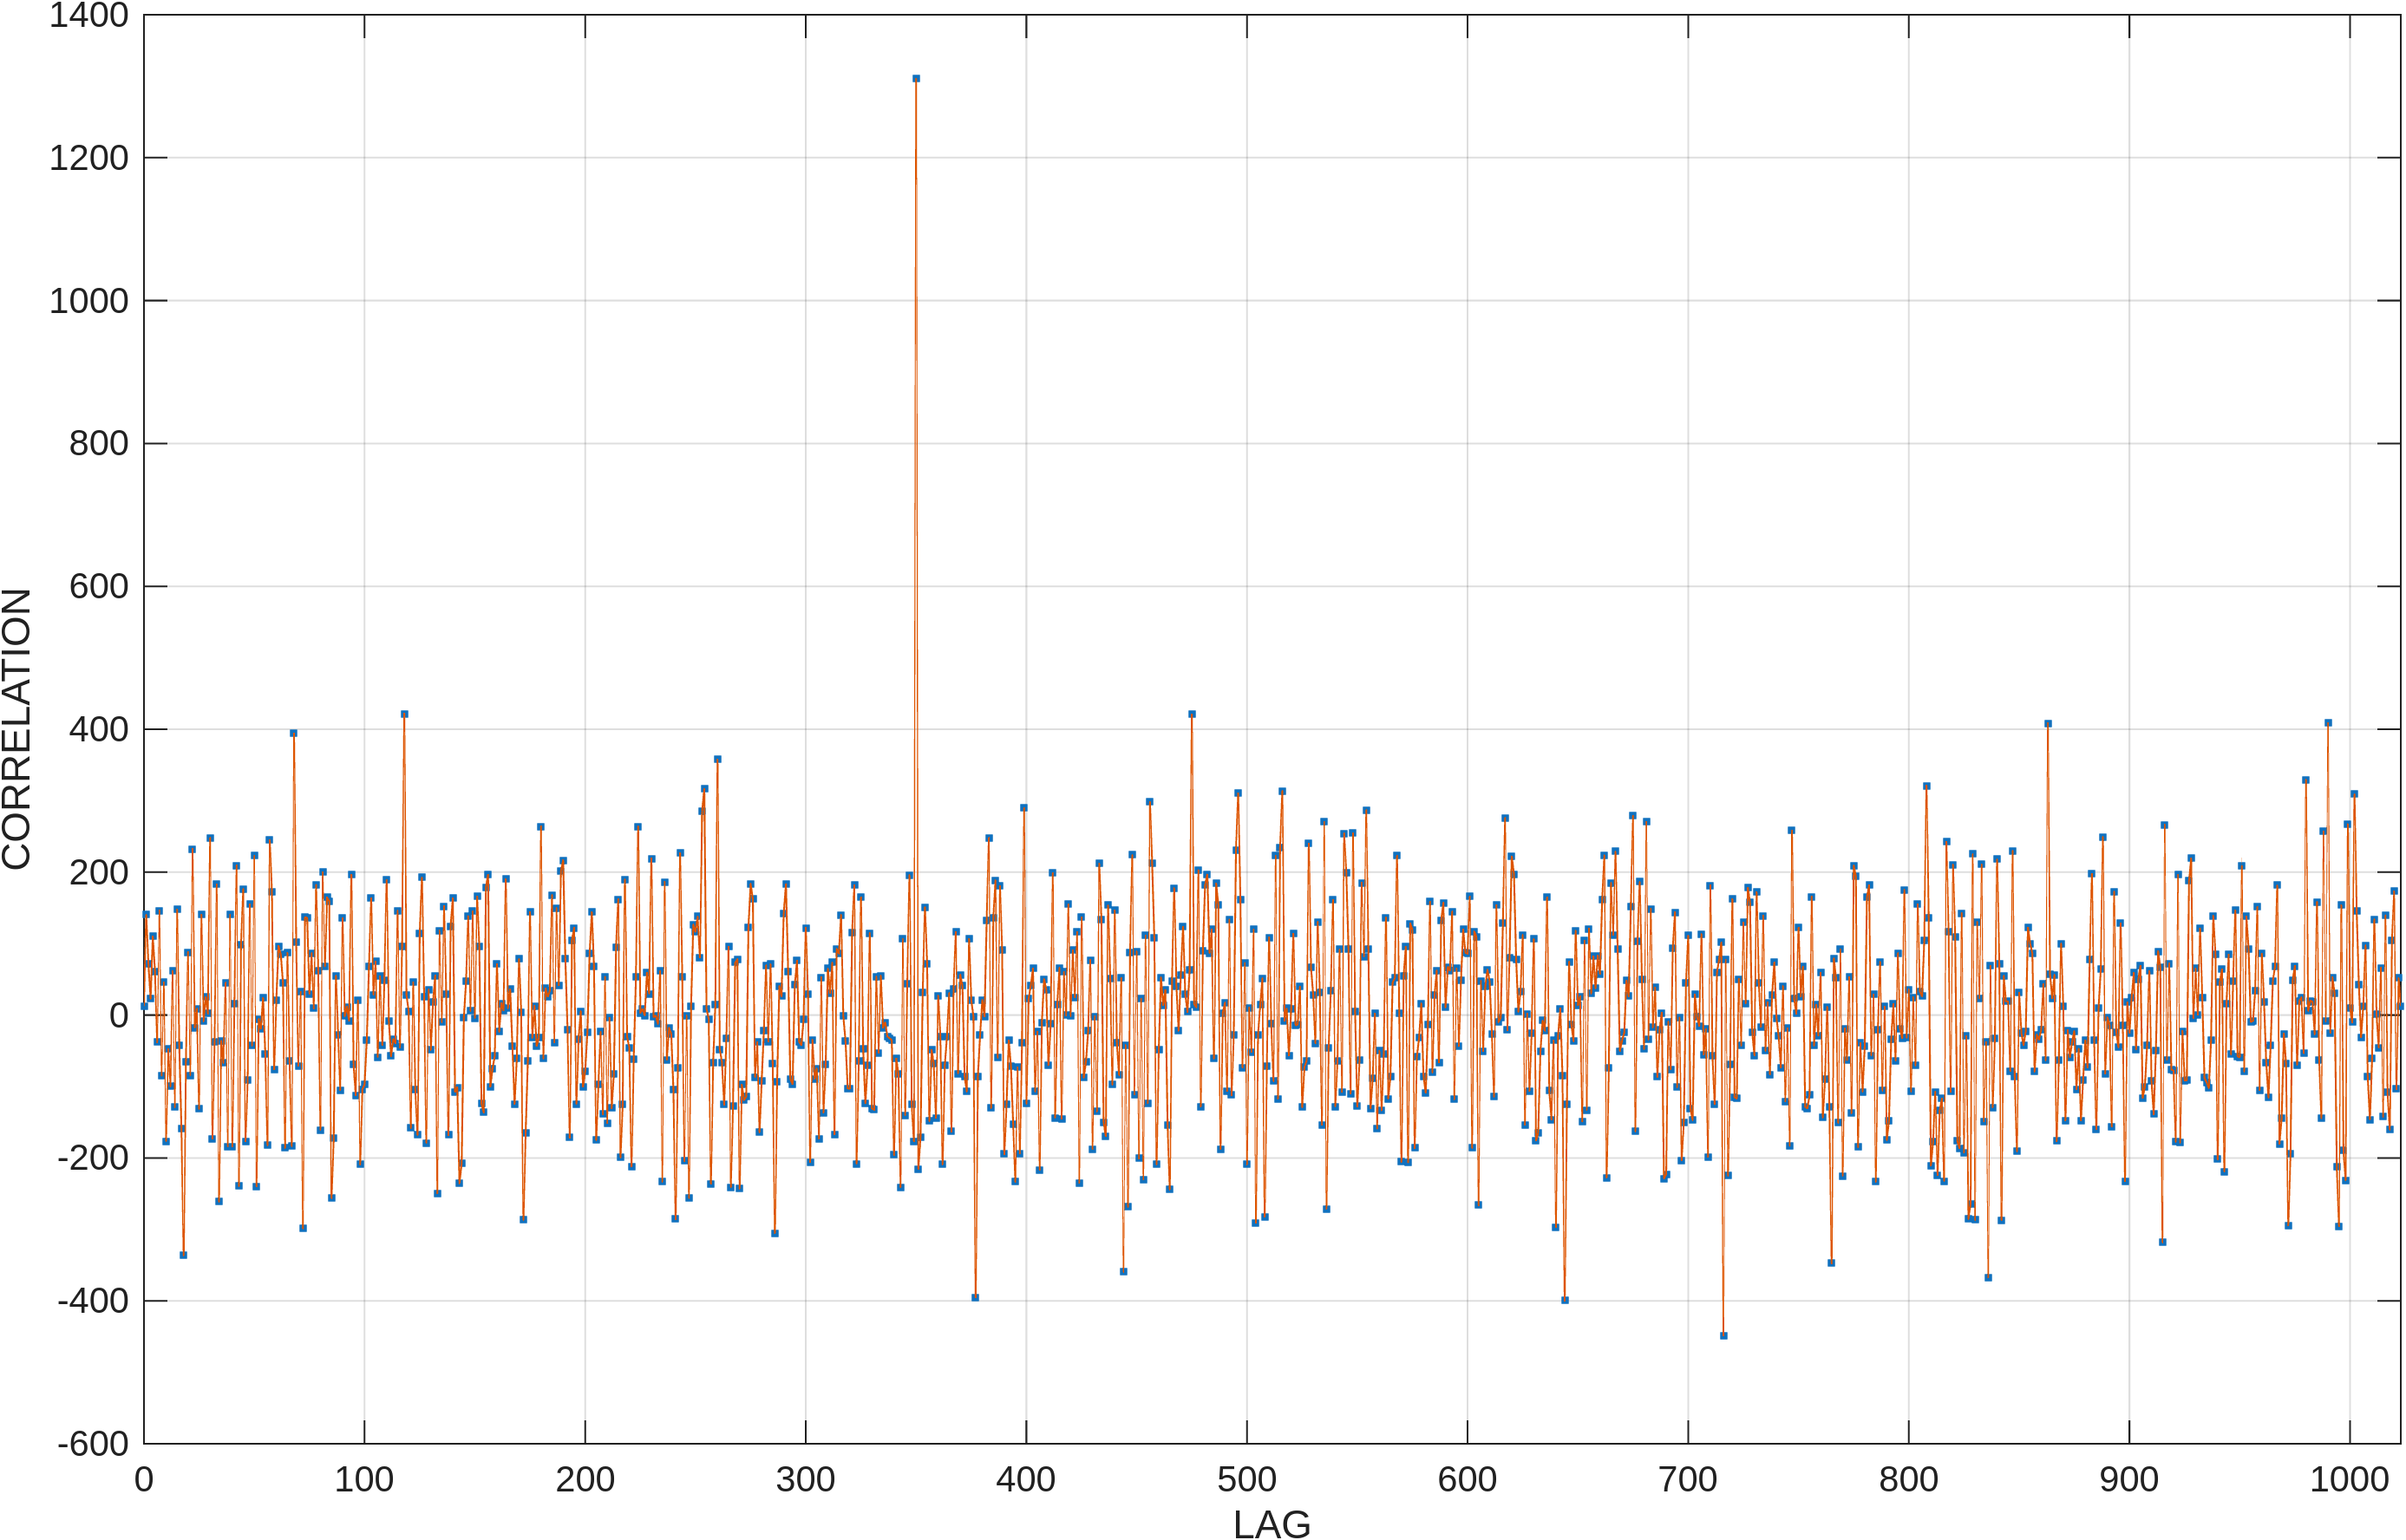
\includegraphics[width=0.8\textwidth]{../PRN5xsum_noise_PRN19_Crosscorrelation.png}
    \caption{PRN Cross Correlation of sum of $x_1,x_2,x_3$ with Noise}
    \label{fig:PRN x1x2x3_noise_plot}
\end{figure}

\hspace*{2em}Taking a look at the results at Figure \ref{fig:PRN x1x2x3_noise_plot},
we do indeed observe that there is a noticable peak at 350 in the lag axis. This is 
where I would expect it to be located, the same logic applies from part (f.), where
there would naturally be a spike at this lag of 350 because that would be auto correlating
with the orinal code of PRN 19 we are examining. I am however rather surprised how based on
Figure \ref{fig:x1x2x3_noise_plot}, noise is comparitively very large compared to the chip values,
and yet the correlated peak is still very prominent despite this large noise being applied.


\end{document}
